% ------------------------------------------------------------------------
%
% -------------------      Plantilla_UIS.tex       -----------------------
%
% ------------------------------------------------------------------------
% ------------------------------------------------------------------------
% ------------------------------------------------------------------------
% Versi�n de plantilla para realizaci�n de informes de trabajo de grado
% construida para uso de la Universidad Industrial de Santander.
%
% Reservados todos los derechos
%
% Bucaramanga, Colombia
%
% Febrero 03 de 2019
%
% ------------------------------------------------------------------------
% ------------------------------------------------------------------------
% ------------------------------------------------------------------------
%
% ------------------------------------------------------------------------
\documentclass[letter,oneside,12pt,spanish]{report}          % Encabezados
% ------------------------------------------------------------------------
\usepackage{uislatexstyleAPA}                           % Libreria UIS APA
% ------------------------------------------------------------------------
% Ingrese en este punto las librer�as espec�ficas de usuario
% ------------------------------------------------------------------------
\usepackage{epsfig}
\usepackage{amsmath}
\usepackage{amssymb}
\usepackage{subfigure}
\usepackage{longtable}
\usepackage{lscape}
\usepackage{float}
\usepackage{listings}
\usepackage{xcolor}
\usepackage{textcomp}
\lstset{
	basicstyle=\ttfamily,
	columns=fullflexible,
	frame=single,
	breaklines=true,
	postbreak=\mbox{\textcolor{red}{$\hookrightarrow$}\space},
}

% ------------------------------------------------------------------------
\begin{document}                                     % Inicio de documento
% ------------------------------------------------------------------------
% Definici�n sil�bica de palabras
% ------------------------------------------------------------------------
\hyphenation{pro-por-cio-nal di-se-�o}
% ------------------------------------------------------------------------
% Titulo resumido del trabajo que aparecer� en cornisa
% ------------------------------------------------------------------------
\title{Definici�n de una infraestructura cloud}
% ------------------------------------------------------------------------
% Elementos previos al contenido del trabajo
% ------------------------------------------------------------------------
% ------------------------------------------------------------------------
%                               Portadilla
% ------------------------------------------------------------------------

\begin{center}

Definici�n de una infraestructura cloud de alta disponibilidad en un entorno distribuido para el despliegue de una plataforma IoT	 \vspace{2.3cm}

Jose David Rojas Aguilar\\ \vspace{2.3cm}

Trabajo de Grado para optar al t�tulo de Ingeniero de Sistemas\\ \vspace{2.3cm}

Director\\
Gabriel Rodrigo Pedraza Ferreira\\
Doctorado en Ciencias de la computaci�n \vspace{2.4cm}

Universidad Industrial de Santander\\
Facultad de Ingenier�as Fisicomec�nicas\\
Escuela de Ingenier�a de sistemas e inform�tica\\
Bucaramanga\\
2019\\


\end{center}

% ------------------------------------------------------------------------
%                             Nota de proyecto
% ------------------------------------------------------------------------

\newpage

\begin{figure}
\begin{center}
\includegraphics[width=1.0\textwidth]{figs/nota}
\end{center}
\end{figure}

% ------------------------------------------------------------------------
%                             Autorizaci�n
% ------------------------------------------------------------------------

\newpage

\begin{figure}
\begin{center}
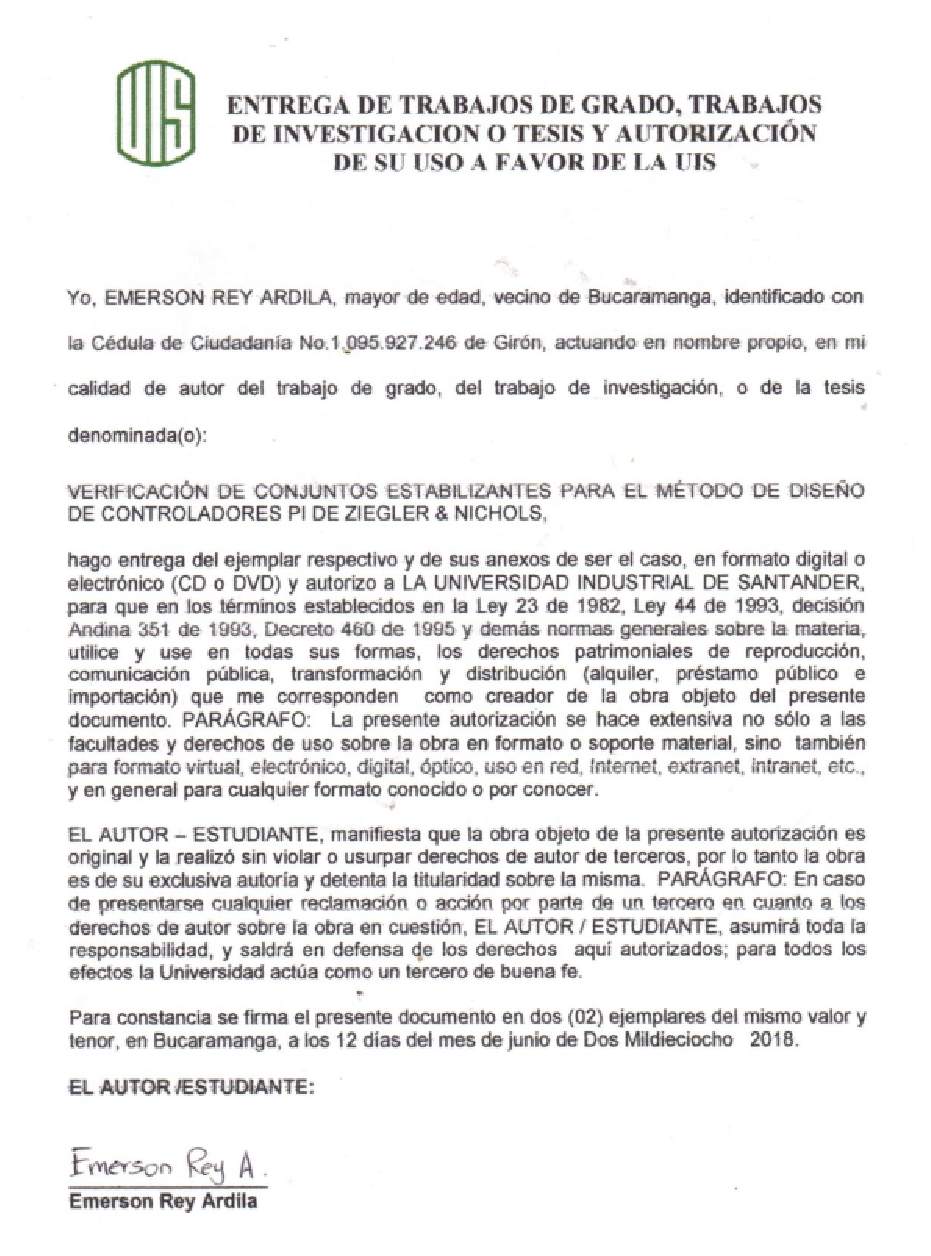
\includegraphics[width=0.9\textwidth]{figs/autoriza}
\end{center}
\end{figure}
% ------------------------------------------------------------------------              % Portadilla, formato de nota y autorizaci�n
% ------------------------------------------------------------------------
% ------------------------------------------------------------------------
% ------------------------------------------------------------------------
% ------------------------------------------------------------------------
%                               Dedicatoria
% ------------------------------------------------------------------------
% ------------------------------------------------------------------------
% ------------------------------------------------------------------------
\chapter*{Dedicatoria}

\noindent Este trabajo viene dedicado para todas aquellas personas que apoyaron el desarrollo
y ejecuci�n de este trabajo de grado.\\

En especial reconozco la permanente presencia de Dios en mi camino de vida.
% ------------------------------------------------------------------------                                    % Dedicatoria
% ------------------------------------------------------------------------
% ------------------------------------------------------------------------
% ------------------------------------------------------------------------
% ------------------------------------------------------------------------
%                             AGRADECIMIENTOS
% ------------------------------------------------------------------------
% ------------------------------------------------------------------------
% ------------------------------------------------------------------------
\chapter*{Agradecimientos}

%\noindent 
% ------------------------------------------------------------------------
\newpage                            % Agradecimientos
% ------------------------------------------------------------------------
\tableofcontents                                      % Tabla de contenido
% ------------------------------------------------------------------------
\listoffigures                         % Lista de figuras, tablas y anexos
\listoftables
\listofanexo
% ------------------------------------------------------------------------
% ------------------------------------------------------------------------
% ------------------------------------------------------------------------
% ------------------------------------------------------------------------
%                                Glosario
% ------------------------------------------------------------------------
% ------------------------------------------------------------------------
% ------------------------------------------------------------------------
\chapter*{Glosario}

\begin{description}
  \item [Actuators] Dispositivo final, l�gico, transforma las se�ales el�ctricas de aviso en la activaci�n de un proceso con la finalidad de generar un efecto sobre un proceso automatizado. 
  \item[Backend] Capa  software  que  se  encarga  de  gestionar  los  datos  de  una  o  varias aplicaciones.
  \item[Continuous deployment] Pr�ctica que consiste en realizar el proceso de despliegue de forma autom�tica al ambiente de producci�n.
  \item[Dataset] Conjunto de datos generados o extra�dos de una fuente para su posterior procesamiento.
  \item[Development \& Operations] Es una pr�ctica de ingenier�a de software que tiene como objetivo automatizar y monitorear las etapas del ciclo de vida del software.
  \item [Gateway] Un gateway en una soluci�n de internet de las cosas puede ser un protocolo gateway desplegado en la nube o un gateway de campo desplegado localmente con otros dispositivos como sensores o actuadores.
  \item[Infraestructura] Conjunto de componentes inform�ticos que permiten mantener un conjunto de aplicaciones al servicio de usuarios.
  \item[Internet de las cosas] Es un sistema de dispositivos de computaci�n interrelacionados con la capacidad de transferir datos a trav�s de una red, sin requerir intervenci�n humana.
  \item[Sensors] Dispositivo capaz de medir una magnitud presente en el ambiente.
  % \item[Sistema de alimentaci�n ininterrumpida] Dispositivo que almacena energ�a para suministrar a equipos en caso de alguna falla el�ctrica.
\end{description}
% ------------------------------------------------------------------------                              % Glosario de t�rminos
% ------------------------------------------------------------------------
% Contenido del Informe
% ------------------------------------------------------------------------
% ------------------------------------------------------------------------
% ------------------------------------------------------------------------
% ------------------------------------------------------------------------
%                                Resumen
% ------------------------------------------------------------------------
% ------------------------------------------------------------------------
% ------------------------------------------------------------------------
\chapter*{Resumen}

\footnotesize{
\begin{description}
  \item[T�tulo:] Definici�n de una infraestructura cloud de alta disponibilidad en un entorno distribuido para el despliegue de una plataforma IoT\astfootnote{Trabajo de grado}
  \item[Autor:] Jose David Rojas Aguilar \asttfootnote{Facultad de Ingenier�as F�sico-Mec�nicas. Escuela de Ingenier�a de sistemas e inform�tica. Director: Gabriel Rodrigo Pedraza Ferreira, Doctor en Ciencias de la Computaci�n.}
  \item[Palabras Clave:] Internet de las cosas, Escalabilidad, Smart Campus, Infraestructura, Cloud, Alta Disponibilidad.
  \item[Descripci�n:] El internet de las cosas (IoT) ha tenido un gran impacto en los �ltimos a�os dentro de la sociedad en diferentes contextos. Una de sus aplicaciones m�s importantes es la mejora de la calidad de vida y el apoyo en el proceso de aprendizaje de los estudiantes dentro de las diferentes universidades. Un reto dentro del IoT es tener una infraestructura capaz de soportar una cantidad masiva de dispositivos enviando informaci�n de forma constante. \\
  
  Este trabajo de investigaci�n se busca dise�ar una arquitectura software para el despliegue de una plataforma IoT en una infraestructura cloud de alta disponibilidad en un entorno distribuido. El proyecto inici� con una fase de exploraci�n con el fin de identificar las herramientas disponibles en el mercado. Luego se definieron unos criterios de selecci�n a nivel t�cnico, unos requisitos de los artefactos a desplegar, un conjunto de m�tricas y un conjunto de pruebas para evaluar el desempe�o de la arquitectura plateada. Despu�s se defini� una arquitectura la cual fue evaluada, en una primera oportunidad, por las pruebas dise�adas durante el proyecto y, finalmente, en una prueba de integraci�n en un caso de uso de la plataforma IoT.
\end{description}}\normalsize
% ------------------------------------------------------------------------                                                % Resumen
% ------------------------------------------------------------------------
% ------------------------------------------------------------------------
% ------------------------------------------------------------------------
%                                Abstract
% ------------------------------------------------------------------------
% ------------------------------------------------------------------------
% ------------------------------------------------------------------------
\chapter*{Abstract}

\footnotesize{
\begin{description}
  \item[Title:] Definition of a cloud infrastructure of high availability in a distributed environment for the deployment of an iot platform\astfootnote{Bachelor Thesis}
  \item[Author:] Jose David Rojas Aguilar\asttfootnote{Faculty of Physical-Mechanical Engineering. School of Systems Engineering and Informatics. Advisor: Gabriel Rodrigo Pedraza Ferreira, PhD in Computer science}
  \item[Keywords:] Infrastructure, Cloud, High availability, Definition, Cluster.
  \item[Description:] The Internet of Things (IoT) has had a strong impact in recent years within society in different contexts. One of its most important applications is the improvement of the quality of life and the support in the learning process of the students in different universities. A challenge in the IoT is to have an infrastructure capable of supporting a massive amount of devices sending information constantly. \\
  
  This research work looks for design software architecture for the deployment of an IoT platform in a high availability cloud infrastructure in a distributed environment. The project began with an exploration phase in order to identify the tools available in the market. Then technical selection criteria were defined, requirements of the artifacts to be deployed, a set of metrics and a set of tests to evaluate the performance of the proposed architecture. An architecture was defined, which was evaluated, at a first opportunity, by the tests designed during the project and, finally, in an integration test in a case of use of the IoT platform.
\end{description}}\normalsize
% ------------------------------------------------------------------------                                               % Abstract
% ------------------------------------------------------------------------
% Cap�tulos
% ------------------------------------------------------------------------
% ------------------------------------------------------------------------
% ------------------------------------------------------------------------
% ------------------------------------------------------------------------
%                              Introducci�n
% ------------------------------------------------------------------------
% ------------------------------------------------------------------------
% ------------------------------------------------------------------------

\nnchapter{Introducci�n}
% ------------------------------------------------------------------------
% ------------------------------------------------------------------------


\noindent La expansi�n de internet y los grandes avances la comunicaci�n entre diferentes dispositivos ha permitido el surgimiento de un nuevo paradigma tecnol�gico: Internet de las cosas (IoT). IoT se define como la infraestructura mundial para la sociedad de la informaci�n, que permite poner diferentes servicios a dispositivos interconectados entre s�, gracias a las tecnolog�as de la informaci�n y comunicaci�n, permitiendo la extracci�n y procesamiento masivo de datos. \\

El internet de las cosas ha tenido un impacto significativo en contextos de diferentes magnitudes. Grandes empresas como Amazon, Microsoft, Google, Cisco, Philips e Intel han invertido millones en investigaci�n, generando diferentes servicios enfocados al hogar, empresas e incluso ciudades. Barcelona es una ciudad pionera en el uso de IoT en sus calles, por ejemplo, la l�nea 9 del metro de Barcelona se ha actualizado con ascensores inteligentes que utilizan los datos en tiempo real para adaptarse a las necesidades de los viajeros lo cual ha logrado disminuir las aglomeraciones y el consumo de energ�a para 30 millones de pasajeros al a�o\citep{BARCELONA2019}. \\

Uno de los campos de aplicaci�n del IoT se encuentra en las universidades con el fin de mejorar la calidad de vida y apoyar el proceso de formaci�n en los estudiantes. La implementaci�n de una soluci�n IoT suele ser una tarea muy compleja que requiere de una infraestructura hardware y software capaz de soportar una cantidad masiva de dispositivos enviando informaci�n de forma continua por lo cual una caracter�stica fundamental dentro de una infraestructura IoT es la alta disponibilidad. \\

En este trabajo de investigaci�n se presenta el dise�o de una infraestructura para el despliegue de una plataforma IoT en una infraestructura cloud de alta disponibilidad en un entorno distribuido con el fin de proveer un entorno que pueda soportar una gran de dispositivos conectados enviado datos de forma masiva. 
   	% Introducci�n
% ------------------------------------------------------------------------
% ------------------------------------------------------------------------
% ------------------------------------------------------------------------
%                              Objetivos
% ------------------------------------------------------------------------
% ------------------------------------------------------------------------
% ------------------------------------------------------------------------

\chapter{Objetivos}
% ------------------------------------------------------------------------
% ------------------------------------------------------------------------

\section*{Objetivo general}

\begin{itemize}
   \item[ ] Analizar las condiciones de estabilidad del conjunto de par�metros PI calculados
   empleando el m�todo de dise�o de controladores de Ziegler \& Nichols.
\end{itemize}

\section*{Objetivos espec�ficos}

\begin{itemize}
    \item[ ] Interpretar las tablas de dise�o de par�metros PI de Ziegler \& Nichols en t�rminos de conjuntos estabilizantes;
    \item[ ] Desarrollar un algoritmo que permita verificar las condiciones de estabilidad para controladores PI dise�ados mediante dicho m�todo;
    \item[ ] Implementar una interfaz para c�lculo de controladores PI a partir de selecci�n de par�metros en el dominio del tiempo, admisibles respecto al conjunto estabilizante correspondiente.
\end{itemize}
% ------------------------------------------------------------------------
% ------------------------------------------------------------------------    % Objetivos
% ------------------------------------------------------------------------
% ------------------------------------------------------------------------
% ------------------------------------------------------------------------
%                                Cap�tulo 2
% ------------------------------------------------------------------------
% ------------------------------------------------------------------------
% ------------------------------------------------------------------------

\chapter{Conjunto estabilizante para sistemas LTI}
% ------------------------------------------------------------------------
\noindent En el presente cap�tulo se formula el conjunto de ecuaciones que delimitan la regi�n de estabilidad (\emph{conjunto estabilizante}) para una planta de segundo orden, compensada con un controlador de tres par�metros ($k$, $\alpha$, $\beta$). Este estudio se realiza haciendo uso del \emph{Criterio de estabilidad de Routh-Hurwitz}. La regi�n de estabilidad del sistema se formula asumiendo $k$ de valor conocido en el plano ($\alpha$, $\beta$) de par�metros del controlador, mediante deducciones anal�ticas y simulaciones num�ricas en MATLAB.
% ------------------------------------------------------------------------

\section{Estabilidad para un sistema LTI}\label{estabsect}
% ------------------------------------------------------------------------
\noindent Considere el sistema de control con realimentaci�n unitaria ilustrado en la Fig. \ref{sistem2ord}. Para este sistema $R(s)$ representa la se�al de entrada, $E(s)$ la se�al de error, $Y(s)$ la se�al de salida, $P(s)$ la funci�n de transferencia de la planta y $C(s)$ la funci�n de transferencia para un controlador de estructura fija y 3 par�metros, dado por:
% ------------------------------------------------------------------------
\begin{equation}
C(s)=\frac{k(s+\alpha)}{\left(s+\beta\right)}.\label{controlador}
\end{equation}\

% ------------------------------------------------------------------------
\begin{figure}[h]
\centering
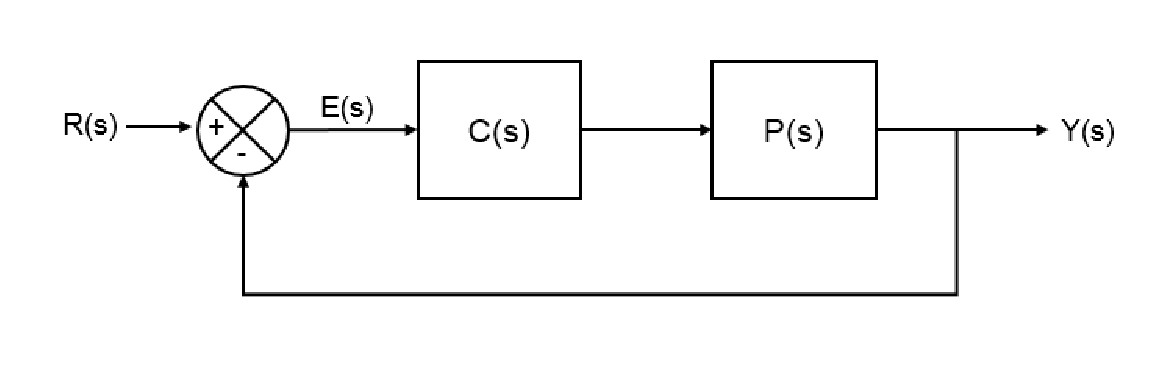
\includegraphics[width=0.5\textwidth]{figs/control_sistem}
\caption{Sistema de control con realimentaci�n unitaria}\label{sistem2ord}
\end{figure}

% ------------------------------------------------------------------------
Para efectos de ilustraci�n, se asumir� una planta gen�rica de segundo orden con un polo en el origen, a partir de:
% ------------------------------------------------------------------------
\begin{equation}
P(s)=\frac{1}{s(s+2)}=\frac{N(s)}{D(s)},\label{planta}
\end{equation}\
% ------------------------------------------------------------------------
definiendo a su vez el siguiente polinomio caracter�stico:
% ------------------------------------------------------------------------
\begin{eqnarray}
\nonumber \delta(s) & = & N(s)[k(s+\alpha)]+D(s)(s+\beta) \\
\nonumber           & = & k(s+\alpha)+s(s+\alpha)(s+\beta)\\
                    & = & s^{3}+(2+\beta)s^{2}+(2\beta+k)s+k\alpha,\label{eqcaract}
\end{eqnarray}\
% ------------------------------------------------------------------------
cuyas ra�ces establecen la estabilidad del sistema.\\

Como es bien sabido, el \emph{Criterio de estabilidad de Routh-Hurwitz} \citep{ogata2010} permite determinar las condiciones para la estabilidad absoluta de un sistema din�mico, mediante un m�todo tabulado que define la posici�n de las ra�ces en el plano, para un polinomio que representa el denominador de la funci�n de transferencia del sistema.\\

As� entonces, se aplica dicho criterio a partir de los siguientes pasos:
% ------------------------------------------------------------------------
\begin{itemize}
% ------------------------------------------------------------------------
% ------------------------------------------------------------------------
% ------------------------------------------------------------------------
\item[1.] \emph{Se escribe el polinomio caracter�stico en la forma $\delta(s) = 0$ y se verifican las condiciones para que todos sus coeficientes sean diferentes de cero y del mismo signo}. De esta manera, asumiendo una convenci�n positiva, los coeficientes de \eqref{eqcaract} ser�n mayores a cero si se cumplen las siguientes condiciones:
$$
\left(2+\beta\right)>0; \quad \left(2\beta+k\right)>0; \quad k\alpha>0,
$$
a partir de lo cual, asumiendo que $k > 0$ es un par�metro constante conocido, las condiciones para estabilidad recaen sobre los par�metros restantes $\left\{\alpha, \beta \right\}$, siendo:
\begin{equation}\label{primera}
\beta > -2; \quad \beta > -\frac{k}{2}; \quad \alpha > 0.
\end{equation}
% ------------------------------------------------------------------------
% ------------------------------------------------------------------------
% ------------------------------------------------------------------------
\item[2.] \emph{Se construye el arreglo de Routh y se analizan los elementos en la primera columna}. \emph{La condici�n necesaria y suficiente para que todas las ra�ces de \eqref{eqcaract} se encuentren en el semiplano izquierdo del plano ``$s$'', es que no existan cambios de signo en la primera columna del arreglo} \citep{ogata2010}. A partir de ello se tiene:
% ------------------------------------------------------------------------
\begin{center}
	\begin{tabular}{ l | c  c  }
		$s^{3}$ 	& 1                        & $\left(2\beta+k\right)$  \\
		$s^{2}$ 	& $\left(2+\beta\right)$   & $k\alpha$                \\
		$s^{1}$ 	& $M$                      & $ 0$                     \\
		$s^{0}$ 	& $k\alpha$                &                          \\
	\end{tabular}
\end{center}
% ------------------------------------------------------------------------
siendo
% ------------------------------------------------------------------------
\begin{eqnarray*}
M & = & \frac{\left(2\beta+k\right)\left(2+\beta\right)-k\alpha}{\left(2+\beta\right)},
\end{eqnarray*}
% ------------------------------------------------------------------------

de lo cual, $M>0$ implica
$$
(2\beta+k)(2+\beta)-k\alpha>0,
$$
puesto que $\left(2+\beta\right)>0$ y as� entonces:
$$
2\beta^{2}+\left(4+k\right)\beta+2k-k\alpha>0.
$$
Despejando $\alpha$ en la expresi�n anterior se obtiene:
% ------------------------------------------------------------------------
\begin{equation}
\alpha < \frac{2}{k}\left(\left(\beta+\frac{\left( k+4\right)}{4}\right)^{2} - \frac{\left(k-4\right)^2}{16}\right),\label{lim_alpha}
\end{equation}

tomando en cuenta que:
\begin{eqnarray*}
\frac{2\beta^{2}+\left(4+k\right)\beta+2k}{k} & = & \frac{2}{k}\left(\beta^{2}+\frac{\left(k+4\right) }{2}\beta+k\right)\\
& = & \frac{2}{k}\left(\beta^{2}+\frac{\left(k+4\right)}{2}\beta+\frac{\left(k+4\right)^2}{16}-\frac{\left(k+4\right)^2}{16}+k\right)\\
& = & \frac{2}{k}\left(\left(\beta+\frac{\left( k+4\right)}{4}\right)^{2} + \frac{16k -\left(k^2+8k+16\right)}{16}\right)\\
& = & \frac{2}{k}\left(\left(\beta+\frac{\left( k+4\right)}{4}\right)^{2} - \frac{\left(k^2-8k+16\right)}{16}\right)\\
& = & \frac{2}{k}\left(\left(\beta+\frac{\left( k+4\right)}{4}\right)^{2} - \frac{\left(k-4\right)^2}{16}\right). \label{stabsetlim}
\end{eqnarray*}
% ------------------------------------------------------------------------
% ------------------------------------------------------------------------
% ------------------------------------------------------------------------
\item[3.] \emph{A partir de las restricciones obtenidas sobre los t�rminos de la primera columna del arreglo de Routh, se determina el rango de valores que asegura para cada par�metro la estabilidad absoluta del sistema}. Por tanto, para $k > 4$ la condici�n que prevalece sobre el par�metro $\beta$ ser�:
    \begin{equation}
    \beta > -2.\label{stabset1}
    \end{equation}
    Asimismo se tiene:
    \begin{equation}
    0 < \alpha < \frac{2}{k}\left(\left(\beta+\frac{\left( k+4\right)}{4}\right)^{2} - \frac{\left(k-4\right)^2}{16}\right).\label{stabset2}
    \end{equation}
% ------------------------------------------------------------------------
\end{itemize}\

% ------------------------------------------------------------------------
\section{Conjunto estabilizante}\label{conjestabsect}
% ------------------------------------------------------------------------
\noindent Dada una estructura de controlador fija $C(s)$ para una planta $P(s)$, el conjunto estabilizante $\mathcal{S}$ se define como todos los posibles controladores $C(s)$ que brindan una soluci�n estable para el sistema realimentado mostrado en la Fig. \ref{sistem2ord}.\\

En este punto es importante resaltar que en la mayor�a de m�todos cl�sicos para el dise�o de controladores, el c�lculo de los par�metros del controlador se realiza sin incluir restricciones expl�citas de estabilidad. En general, un dise�o viene acompa�ado por pruebas de verificaci�n no s�lo para las condiciones de operaci�n del sistema controlado sino tambi�n para su estabilidad, constituyendo procedimientos iterativos muchas veces del tipo ensayo y error.\\

En otras palabras, los m�todos de dise�o se formulan para cumplir con condiciones de desempe�o sobre un sistema controlado estable, pero no toman en cuenta que a�n cuando matem�ticamente el controlador pueda satisfacer el problema, existe un conjunto restringido de par�metros de control que aseguran la estabilidad del sistema.\\

El conjunto establizante $\mathcal{S}$ es f�cil de definir. Por ejemplo, para la combinaci�n de planta y controlador dada por las ecuaciones \eqref{controlador}-\eqref{planta} en la Secci�n \ref{estabsect}, dicho conjunto puede escribirse como:
\begin{equation}
\mathcal{S} = \left\{\left(k, \alpha,\beta\right): \: \text{\eqref{stabset1} y \eqref{stabset2} se satisfagan simult�neamente} \right\}.\label{stabseteq}
\end{equation}

El conjunto estabilizante $\mathcal{S}$ es dificil de calcular. Para sistemas de bajo orden, el \emph{criterio de estabilidad de Routh-Hurwirtz} puede ser empleado seg�n ilustrado en la Secci�n \ref{estabsect}. Sin embargo, para un orden elevado la cantidad de expresiones no lineales que se requiere combinar para determinar los rangos de par�metros estables justifican la utilizaci�n de m�todos computacionales refinados. El \emph{m�todo de la signatura} propuesto por Keel y Bhattacharyya es una opci�n viable para estos casos \citep{keel2008}.

% ------------------------------------------------------------------------
\subsection{Incidencia de $\mathcal{S}$ en la estabilidad de un lazo de control}\label{lazoestable}
% ------------------------------------------------------------------------
\noindent Para verificar la importancia del conjunto estabilizante, considere el problema de dise�o de un compensador $C(s)$ de la forma \eqref{controlador} para el sistema $P(s)$ definido en \eqref{planta}, de manera tal que el sistema compensado y realimentado como en la Fig. \ref{sistem2ord} exhiba una respuesta escal�n con las siguientes caracter�sticas din�micas:
% ------------------------------------------------------------------------
\begin{equation}
M_p \approx 0\%; \quad t_s|_{2\%} \approx 0.5 \: [s].\label{spec}
\end{equation}\
% ------------------------------------------------------------------------

Inicialmente, se deben traducir las especificaciones de respuesta temporal dadas en \eqref{spec} al dominio de la frecuencia. A partir de ello, los polos deseados para el sistema compensado corresponden con:
% ------------------------------------------------------------------------
\begin{equation}
s = -8.231 \pm 0j \label{polo}.
\end{equation}\
% ------------------------------------------------------------------------

Ahora bien, evaluando este valor para ``$s$'' en $P(s)$, se verifica una deficiencia angular de:
% ------------------------------------------------------------------------
\begin{equation}
\angle C(s) = 180�,
\end{equation}
% ------------------------------------------------------------------------
que a su vez corresponde con la contribuci�n de fase que debe aportar el compensador en el polo deseado. A partir de ello, la localizaci�n para el polo y el cero del compensador se realiza empleando el siguiente an�lisis:
% ------------------------------------------------------------------------
\begin{itemize}
\item[-] Para obtener $180�$ de fase en el compensador, el cociente resultante debe ser un n�mero real negativo teniendo en cuenta el caracter real del polo deseado;
\item[-] Posteriormente se selecciona una distribuci�n en el eje real negativo para la localizaci�n del polo deseado y el polo y el cero del compensador, que conserve una simetr�a dada por un factor:
    $$
    \gamma = \frac{s}{5} \approx \frac{5}{3},
    $$
    en modo tal que:
    $$
    \alpha = \gamma s \approx 13.21, \quad \beta = \frac{s}{\gamma} \approx 4.84;
    $$
\item [-] Por �ltimo se determina la ganancia $k$ del compensador, como aquel valor que satisface
la condici�n de magnitud para el lugar geom�trico de las ra�ces:
% ------------------------------------------------------------------------
\begin{equation}
\left| \frac{k(s+13.21)}{s(s+2)(s+4.84)} \right|_{s=-8.231 \pm 0j}  =  1,
\end{equation}\
% ------------------------------------------------------------------------
a partir de lo cual $k \approx 34.93$.
% ------------------------------------------------------------------------
\end{itemize}\

% ------------------------------------------------------------------------
Una vez dise�ado el compensador, se procede a verificar el desempe�o del sistema controlado
empleando herramientas de simulaci�n. Es as� como la Fig. \ref{examp_inestable} muestra
la respuesta temporal ante un est�mulo de tipo escal�n unitario, calculada empleando el \emph{Control System Toolbox} de MATLAB\circledR~en el sistema compensado y realimentado,
siendo sin embargo de naturaleza inestable. A partir de lo anterior, surge la pregunta: �Por qu� un dise�o que se realiza empleando apropiadamente las herramientas matem�ticas, conduce a un sistema inestable?\\
% ------------------------------------------------------------------------
\begin{figure}[h]
\centering
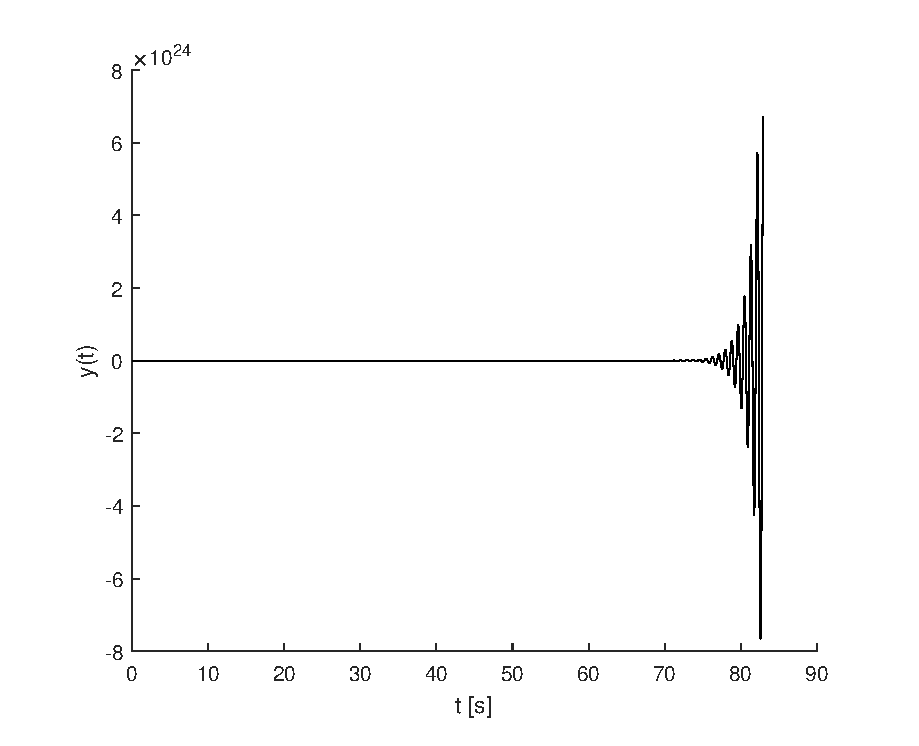
\includegraphics[width=0.5\textwidth]{figs/step_inestab}
\caption[Respuesta escal�n sistema compensado con inestabilidad]{Respuesta escal�n de sistema compensado manifestando inestabilidad}\label{examp_inestable}
\end{figure}

% ------------------------------------------------------------------------
La respuesta para este interrogante se explica f�cilmente a partir de \eqref{stabseteq}, justificando que los requerimientos dados en \eqref{spec} no son viables para la estructura del compensador seleccionada, seg�n se detalla a continuaci�n.

% ------------------------------------------------------------------------
\subsection{Escenarios din�micos viables en $\mathcal{S}$ para el sistema compensado}
% ------------------------------------------------------------------------
\noindent El conjunto estabilizante $\mathcal{S}$ definido en \eqref{stabseteq} depende de las inecuaciones \eqref{stabset1} y \eqref{stabset2}, establecidas a su vez para $k > 0$.\\

De los resultados presentados para el c�lculo del compensador se observa que $k = 34.93$ satisface la �ltima premisa. Por tanto, el controlador ser� estable si tanto $\alpha$ como $\beta$ satisfacen para este valor de $k$, las desigualdades que relacionan los elementos en la primera columna del arreglo de Routh.\\

As� entonces, reemplazando \eqref{primera}-\eqref{lim_alpha} para $k = 34.93$ en \eqref{stabset1} y \eqref{stabset2}, se obtiene:
% ------------------------------------------------------------------------
\begin{eqnarray*}
    \beta &=& 4.84\\
          &>& -2;\\
    \alpha &=& 13.21\\
           &>& 0\\
           & \nless& \frac{2}{34.93}\left(\left(4.84+\frac{\left( 34.93+4\right)}{4}\right)^{2} - \frac{\left(34.93-4\right)^2}{16}\right)\\
           & \nless& 8.73,
\end{eqnarray*}
% ------------------------------------------------------------------------
de donde la �ltima desigualdad muestra la raz�n por la cual el controlador calculado representa un sistema realimentado inestable.\\

De hecho, es posible graficar el plano de par�metros ($\alpha$, $\beta$) que representa los controladores con estructura \eqref{controlador} que para $k = 34.93$
garantizan la estabilidad del sistema controlado y realimentado. Dicha gr�fica se presenta en la Fig. \ref{conjestab1}, siendo el interior de la regi�n gris
el conjunto estabilizante $\mathcal{S}$, mientras el tri�ngulo indica el controlador calculado en la Secci�n \ref{lazoestable} evidenciando su condici�n de
realizaci�n inestable para el sistema.\\
% ------------------------------------------------------------------------

\begin{figure}[h]
\centering
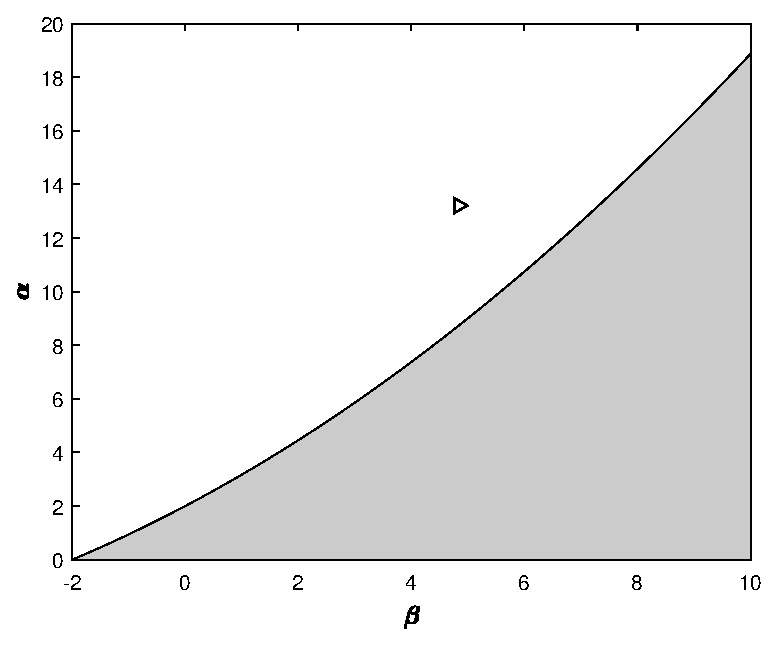
\includegraphics[width=0.5\textwidth]{figs/stab_set1}
\caption{Conjunto estabilizante en el plano ($\alpha$, $\beta$) para $k = 34.93$}\label{conjestab1}
\end{figure}
% ------------------------------------------------------------------------

M�s interesante a�n es transformar dicho conjunto estabilizante en t�rminos de par�metros del controlador hacia un espacio de especificaciones de desempe�o. Por ejemplo, observe en la Fig. \ref{Mp-ts} el plano ($M_p$, $t_s$) equivalente para el conjunto estabilizante mostrado en la Fig. \ref{conjestab1}.\\

De este diagrama se observa la manera en la cual los par�metros de desempe�o requeridos para el dise�o presentado en la Secci�n \ref{lazoestable}, no forman parte de los escenarios din�micos viables en el conjunto estabilizante para el sistema compensado. Visualmente se observa una discontinuidad del conjunto $\mathcal{S}$ al ser mapeado desde el plano ($\alpha$, $\beta$) hacia el plano ($M_p$, $t_s$). Un an�lisis detallado del efecto anterior involucra \emph{topolog�a matem�tica}, superando los alcances del presente trabajo de grado.\\

% ------------------------------------------------------------------------

\begin{figure}[h]
\centering
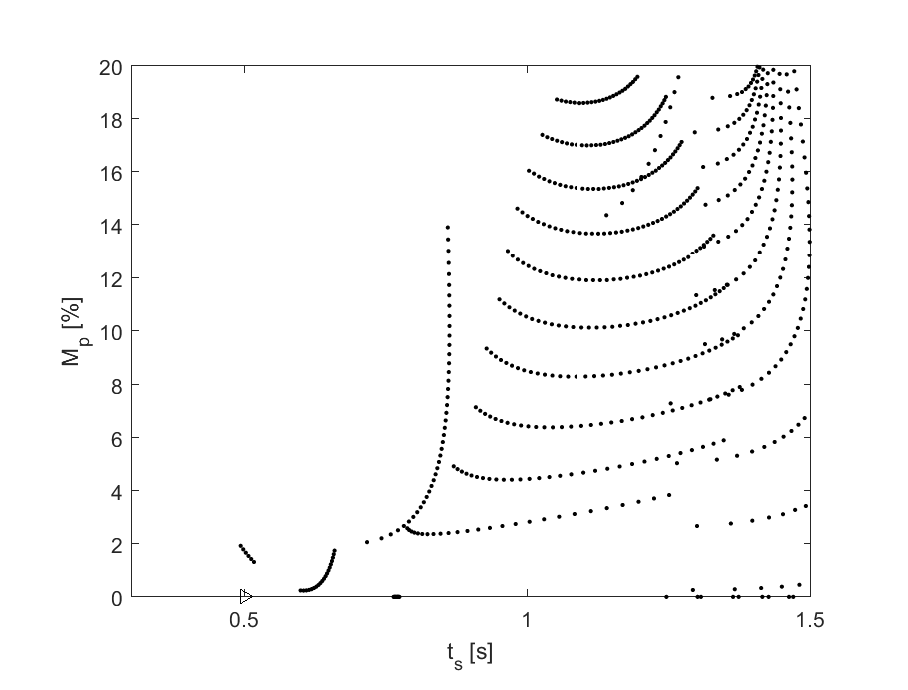
\includegraphics[width=0.7\textwidth]{figs/Mp_ts}
\caption{Conjunto estabilizante en el plano ($M_p$, $t_s$) para $k = 34.93$}\label{Mp-ts}
\end{figure}
% ------------------------------------------------------------------------

Por tanto, dada la dificultad matem�tica que implica un mapeo anal�tico entre el conjunto estabilizante $\mathcal{S}$ y los par�metros de una respuesta escal�n, el plano presentado en la Fig. \ref{Mp-ts} fue generado empleando simulaci�n de fuerza bruta (es decir, punto a punto) a partir de las funciones del \emph{Control Systems Toolbox} de MATLAB\circledR.\\

De esta manera es posible realizar una selecci�n visual para los par�metros del controlador (\emph{m�todo gr�fico de dise�o}) a partir de una elecci�n de las especificaciones de desempe�o requeridas en la respuesta escal�n, al interior del conjunto admisible dado en la Fig. \ref{Mp-ts}\\

La Fig. \ref{respuestas} ilustra la selecci�n para varios escenarios din�micos al interior de la regi�n de estabilidad, con su correspondiente mapeo al plano de par�metros del controlador.\\
% ------------------------------------------------------------------------
\begin{figure}
\centering
	\subfigure[$M_p = 53.38; \: t_s = 3.60$]{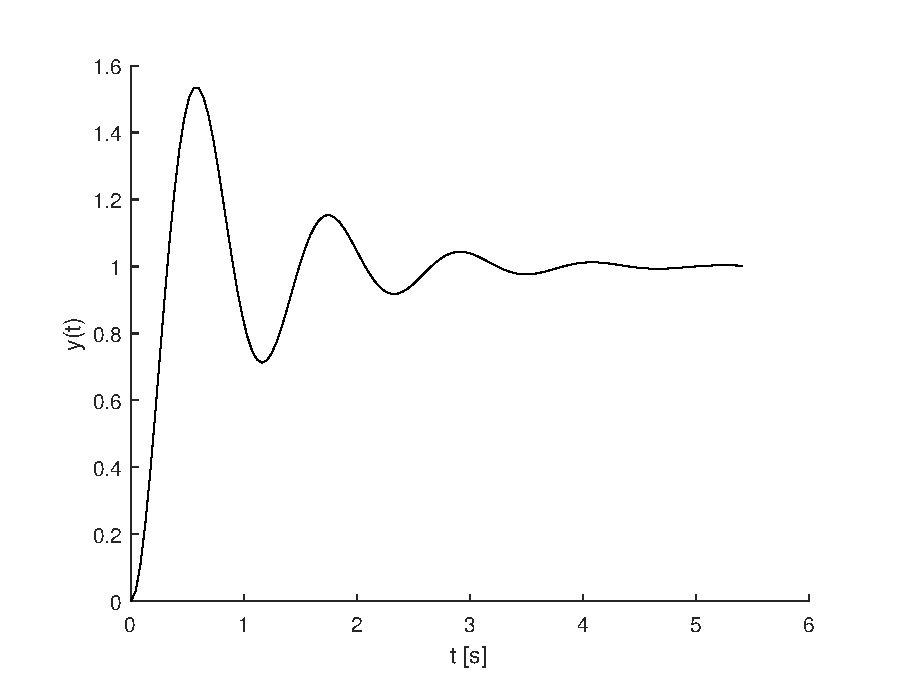
\includegraphics[width=0.45\textwidth]{Figs/step_E1}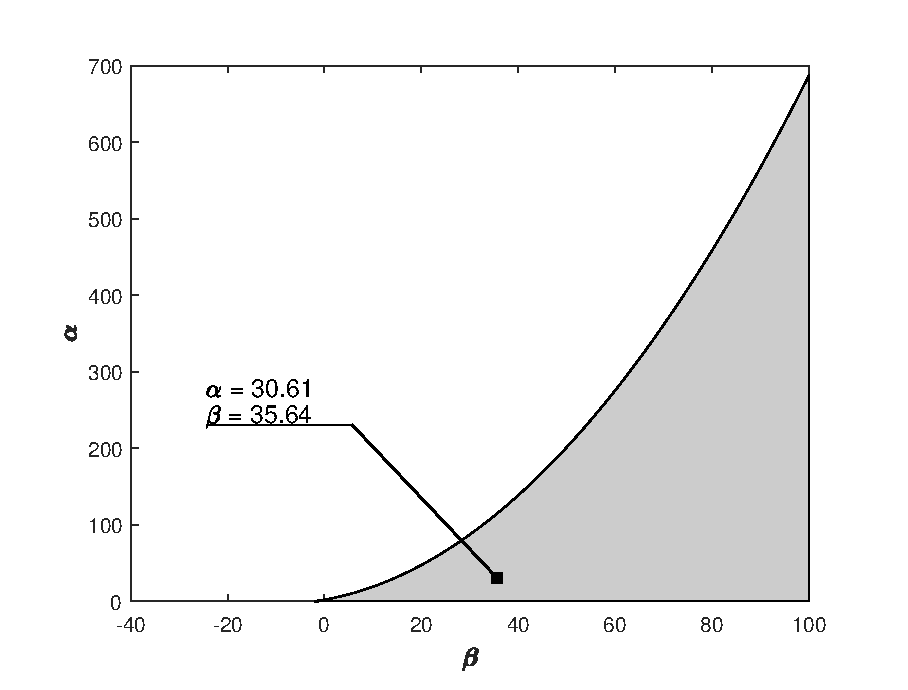
\includegraphics[width=0.45\textwidth]{Figs/stab_set_E1}}
	\subfigure[$M_p = 70.76; \: t_s = 4.59$]{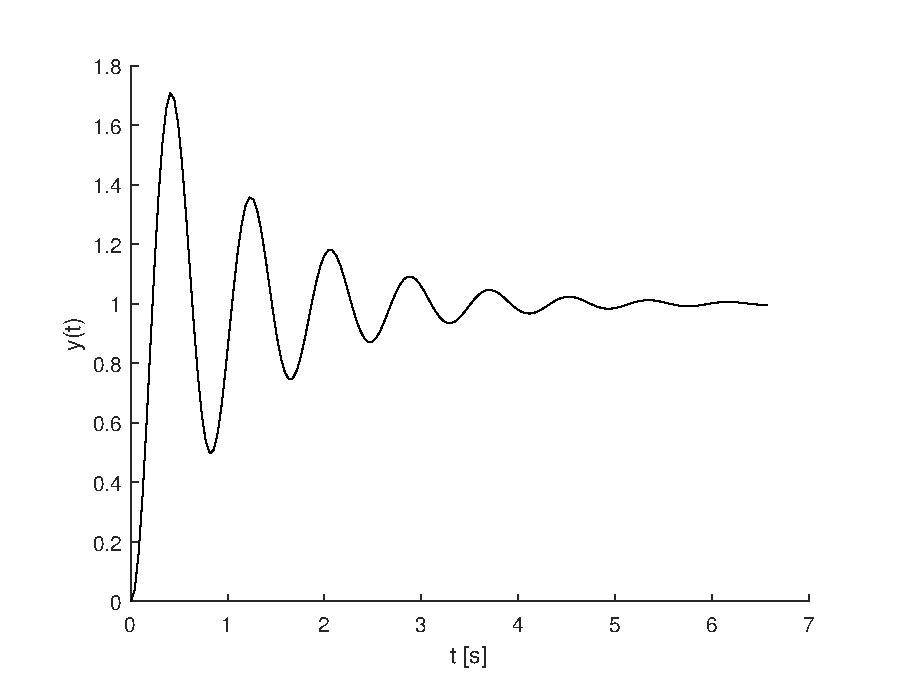
\includegraphics[width=0.45\textwidth]{Figs/step_E2}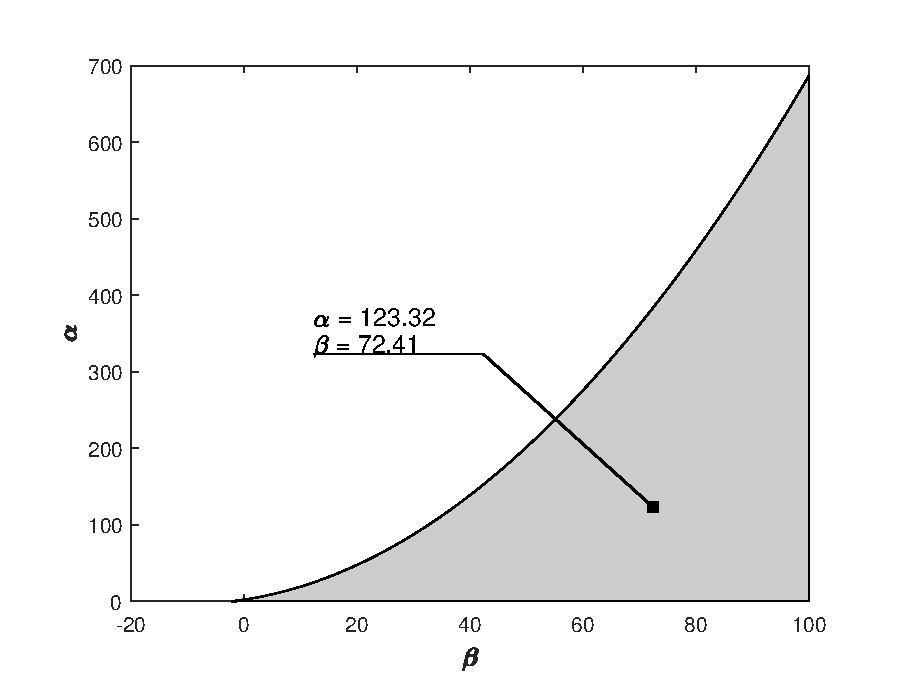
\includegraphics[width=0.45\textwidth]{Figs/stab_set_E2}}
	\subfigure[$M_p = 84.76; \: t_s = 6.85$]{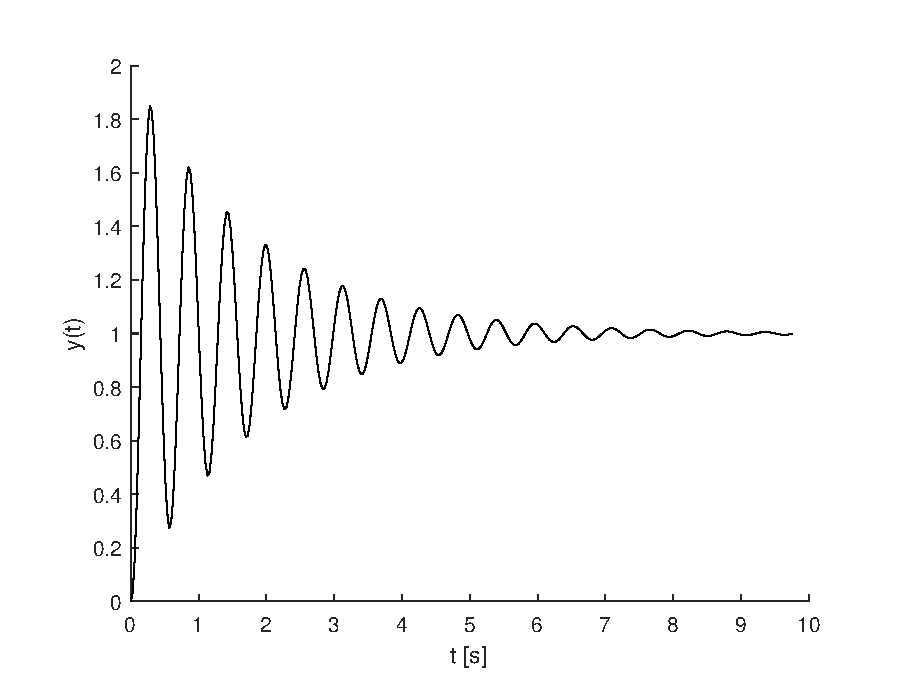
\includegraphics[width=0.45\textwidth]{Figs/step_E3}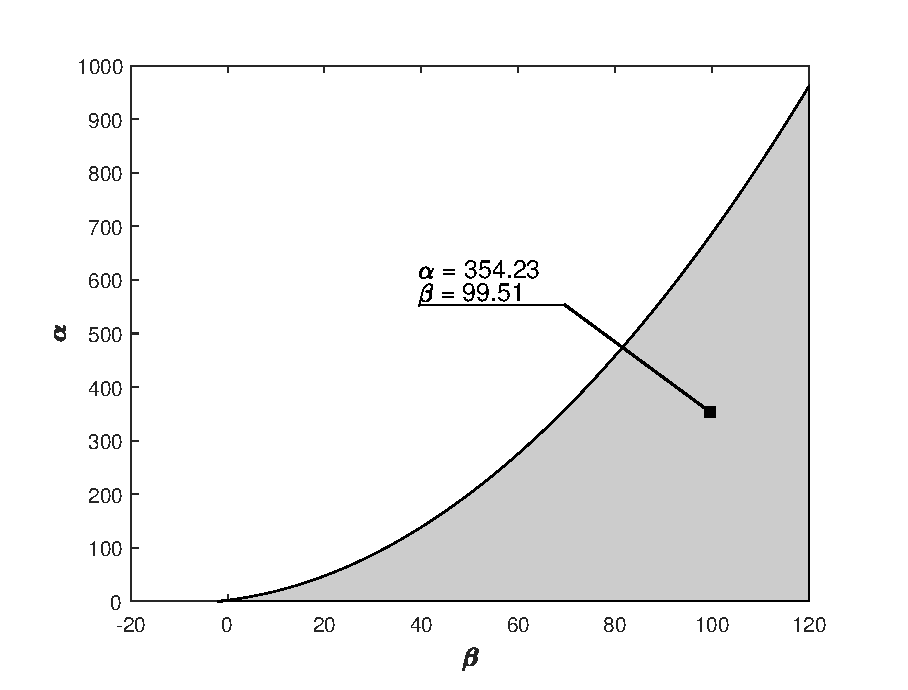
\includegraphics[width=0.45\textwidth]{Figs/stab_set_E3}}
\caption[Respuesta din�mica y controlador en $\mathcal{S}$ del plano ($M_p$, $t_s$)]{Respuesta din�mica y controlador correspondiente para diferentes especificaciones al interior de $\mathcal{S}$ en el plano ($M_p$, $t_s$)}\label{respuestas}
\end{figure}

% ------------------------------------------------------------------------
A partir de lo anterior, pueden emplearse herramientas computacionales para realizar, de manera gr�fica, el c�lculo de un compensador de estructura predeterminada para una planta conocida y con base en el conjunto de especificaciones de desempe�o admisible proporcionadas por el conjunto estabilizante, seg�n se detalla en la siguiente secci�n.

% ------------------------------------------------------------------------
\section{Dise�o gr�fico de controladores a partir del c�lculo de $\mathcal{S}$}\label{interfazsect}
% ------------------------------------------------------------------------
% ------------------------------------------------------------------------
\noindent Tomando en cuenta la alta capacidad de c�lculo y portabilidad de las herramientas computacionales actuales, resulta simple aceptar que las dificultades anal�ticas en la determinaci�n de par�metros de control puedan ser reducidas ostensiblemente a partir de paquetes como MATLAB, que integra funciones optimizadas para aproximar con muy alta precisi�n los valores de variables importantes en un sistema de control realimentado, ante simulaci�n para diversos escenarios de operaci�n.\\

Tomando en cuenta lo anterior, se construy� una interfaz para realizar el dise�o de controladores simples (i.e. compensadores en adelanto o en atraso), a partir de un enfoque gr�fico basado en el c�lculo del conjunto estabilizante para sistemas \emph{SISO LTI}. El dise�o de la interfaz se presenta a continuaci�n empleando como base la descripci�n propuesta por Roa y Ayala en \citep{roa_ayala2016} para este tipo de desarrollos.

% ------------------------------------------------------------------------
\subsection{Descripci�n general de requerimientos}
% ------------------------------------------------------------------------
\noindent Se requiere construir una interfaz de software que permita dise�ar un controlador de estructura simple pre-establecida, a partir de informaci�n del conjunto admisible de par�metros de respuesta din�mica, calculados con base en el conjunto estabilizante $\mathcal{S}$ para un sistema realimentado de manera negativa y unitaria. La interfaz deber� permitir modificar la ganancia $k$ de baja frecuencia del controlador, as� como los rangos de variaci�n del par�metro $\beta$ y la resoluci�n de puntos para el conjunto estabilizante calculado, permitiendo visualizar dicho conjunto en el plano $\left(\alpha,\beta\right)$, su mapeo correspondiente hacia el plano de par�metros de respuesta $\left(M_p, t_s \right)$ y la respuesta escal�n del sistema realimentado para un punto arbitrario dentro de $\mathcal{S}$.

% ------------------------------------------------------------------------
\subsubsection{Nivel superior de detalle}
% ------------------------------------------------------------------------
\noindent Posterior a la descripci�n (en palabras) de los requerimientos del sistema (interfaz), se procede a  crear un diagrama general de entradas y salidas a manera de nivel superior de detalle. Dicha representaci�n se muestra en la Fig. \ref{Nsuperior}.
% ------------------------------------------------------------------------
\begin{figure}[h]
\centering
\includegraphics[width=0.7\textwidth]{figs/Nivel_superior}
\caption[Nivel superior de detalle para desarrollo de interfaz]{Representaci�n de nivel superior de detalle para desarrollo de interfaz}\label{Nsuperior}
\end{figure}
% ------------------------------------------------------------------------

\subsubsection{Partici�n de primer nivel}
% ------------------------------------------------------------------------
\noindent Una primera partici�n se logra con la incorporaci�n del bloque que realiza el c�lculo del conjunto estabilizante $\mathcal{S}$, mediante evaluaci�n de las expresiones \eqref{stabset1}, \eqref{stabset2} y \eqref{stabseteq}.\\
% ------------------------------------------------------------------------
\begin{figure}[h]
\centering
\includegraphics[width=1.0\textwidth]{figs/Primer_nivel}
\caption[Primer nivel de detalle para desarrollo de interfaz]{Representaci�n de primer nivel de partici�n para desarrollo de interfaz}\label{Nprimer}
\end{figure}\
% ------------------------------------------------------------------------

Asimismo, los resultados en esta etapa son la informaci�n de entrada a un nuevo bloque encargado de construir la representaci�n gr�fica del conjunto estabilizante en el espacio de par�metros $\left(M_p, t_s \right)$. Lo anterior se realiza en una secuencia de dos pasos: \emph{1)} se calculan las respuestas escal�n $y(t)$ para el sistema realimentado con cada uno de los par�metros de controlador dados por $\mathcal{S}$ y \emph{2)} se determina el valor correspondiente en el plano $\left(M_p, t_s \right)$ para cada caso.\\

Con esta informaci�n, el usuario puede proceder a seleccionar un punto admisible $\left(M_p^*, t_s^* \right)$, que posteriormente es representado en su versi�n equivalente de par�metros del controlador deseado $\left(\alpha^*,\beta^* \right)$. Finalmente, se calcula para este punto la respuesta escal�n $y^*(t)$ para el sistema realimentado.\\

De esta manera, el primer nivel de partici�n se configura con la uni�n de los anteriores subprocesos, tal y como se ilustra en la Fig. \ref{Nprimer}.

% ------------------------------------------------------------------------
\subsubsection{Particiones de segundo nivel}
% ------------------------------------------------------------------------
\noindent A su vez, cada uno de los subprocesos descritos en el �tem anterior, se descompone en etapas constitutivas fundamentales seg�n se describe a continuaci�n:
% ------------------------------------------------------------------------
\begin{itemize}
% ------------------------------------------------------------------------
\item[-] \emph{C�lculo de $\mathcal{S}$}: para determinar el conjunto estabilizante se debe establecer para un $k$ dado y un intervalo de variaci�n conocido para $\beta$, el rango de $M$ valores para la variable $\alpha$ que satisface las restricciones impuestas por las ecuaciones \eqref{stabset1}, \eqref{stabset2} y \eqref{stabseteq}. El esquema para estas subrutinas se muestra en la Fig. \ref{Nsegundo1};
\item[-] \emph{C�lculo respuesta escal�n a partir de $\left(\alpha,\beta\right)$}: una vez calculado $\mathcal{S}$, es posible evaluar cada punto $\left(\alpha,\beta\right)$ en la estructura de control realimentado mostrada en la Fig. \ref{sistem2ord}. De esta manera puede calcularse, a trav�s de comandos del \emph{Control System Toolbox} de MATLAB, la respuesta escal�n para el sistema. El esquema para estas subrutinas se muestra en la Fig. \ref{Nsegundo2};
\item[-] \emph{Elecci�n de punto admisible en $\left(M_p, t_s \right)$}: a trav�s de selecci�n gr�fica el usuario seleccionar� un punto de inter�s $\left(\bar{M_p}, \bar{t_s} \right)$. Posteriormente, se deber� verificar si dicho punto pertenece al conjunto de par�metros admisibles $\left(M_p, t_s \right)$. En caso afirmativo, el punto se denominar� $\left(M_p^*, t_s^* \right)$. El esquema para estas subrutinas se muestra en la Fig. \ref{Nsegundo3};
\item[-] \emph{Conversi�n punto $\left(M_p^*, t_s^* \right)$ a punto $\left(\alpha,\beta\right)$ dentro de $\mathcal{S}$}: tomando en cuenta que los planos $\left(M_p, t_s \right)$ y $\left(\alpha,\beta\right)$ poseen las mismas dimensiones y son una relaci�n uno a uno, la posici�n del punto $\left(M_p^*, t_s^* \right)$ equivale al conjunto de par�metros $\left(\alpha^*,\beta^* \right)$ del controlador que lo produce. El esquema para estas subrutinas se muestra en la Fig. \ref{Nsegundo4}.
% ------------------------------------------------------------------------
\end{itemize}
% ------------------------------------------------------------------------
\begin{figure}[h]
\centering
\includegraphics[width=0.8\textwidth]{figs/Segundo_Nivel_Sub_1}
\caption[Subproceso de \emph{C�lculo de $\mathcal{S}$}]{Representaci�n de segundo nivel de partici�n para subproceso de \emph{C�lculo de $\mathcal{S}$}}\label{Nsegundo1}
\end{figure}
% ------------------------------------------------------------------------
\begin{figure}[h]
\centering
\includegraphics[width=0.8\textwidth]{figs/Segundo_Nivel_Sub_2}
\caption[Subproceso de \emph{C�lculo respuesta escal�n a partir de $\left(\alpha,\beta\right)$}]{Representaci�n de segundo nivel de partici�n para subproceso de \emph{C�lculo respuesta escal�n a partir de $\left(\alpha,\beta\right)$}}\label{Nsegundo2}
\end{figure}
% ------------------------------------------------------------------------
\begin{figure}[h]
\centering
\includegraphics[width=0.8\textwidth]{figs/Segundo_Nivel_Sub_3}
\caption[Subproceso de \emph{Elecci�n de punto admisible en $\left(M_p, t_s \right)$}]{Representaci�n de segundo nivel de partici�n para subproceso de \emph{Elecci�n de punto admisible en $\left(M_p, t_s \right)$}}\label{Nsegundo3}
\end{figure}
% ------------------------------------------------------------------------
\begin{figure}[h]
\centering
\includegraphics[width=0.8\textwidth]{figs/Segundo_Nivel_Sub_4}
\caption[Subproceso de \emph{Conversi�n $\left(M_p^*, t_s^* \right)$ a $\left(\alpha,\beta\right)$}]{Representaci�n de segundo nivel de partici�n para subproceso de \emph{Conversi�n punto $\left(M_p^*, t_s^* \right)$ a punto $\left(\alpha,\beta\right)$ dentro de $\mathcal{S}$}}\label{Nsegundo4}
\end{figure}
% ------------------------------------------------------------------------

El esquema definitivo para las etapas que constituyen la interfaz, implica la combinaci�n de los esquemas presentados en las Figs. \ref{Nprimer} y \ref{Nsegundo1}-\ref{Nsegundo4}.

% ------------------------------------------------------------------------
\subsection{Selecci�n de herramienta para implementaci�n}
% ------------------------------------------------------------------------
\noindent A partir del diagrama obtenido en la Fig. \ref{Nprimer}, es claro que el coraz�n de la interfaz a ser dise�ada es la rutina que calcula los par�metros de respuesta escal�n en el sistema compensado para cada punto de prueba. Como ya mencionado, estas tareas facilitan su ejecuci�n empleando los comando del \emph{Control System Toolbox} de MATLAB. Por tanto, se considera a dicha herramienta como la primera opci�n para desarrollar la interfaz de software requerida.\\

Mas a�n, MATLAB posee adem�s de la consola de comandos y el entorno de programaci�n gr�fico SIMULINK, un entorno para el desarrollo de interfaces de usuario denominado GUIDE (Graphical User Interface Development Environment).\\

Tomando en cuenta lo anterior, se selecciona MATLAB \emph{vR2017a} para construir la interfaz de usuario que satisface los requerimientos de dise�o ilustrados en los diagramas de nivel de partici�n previamente presentados.

% ------------------------------------------------------------------------
\subsection{Descripci�n de interfaz dise�ada}
% ------------------------------------------------------------------------
\begin{figure}
\centering
\includegraphics[width=1.0\textwidth]{figs/interfaz}
\caption{Presentaci�n final para interfaz desarrollada}\label{interfaz}
\end{figure}
% ------------------------------------------------------------------------

\noindent Procediendo con el dise�o, se realiza codificaci�n en MATLAB para la combinaci�n de los diagramas de bloques de las Figs. \ref{Nprimer}-\ref{Nsegundo4}, asumiendo las siguientes \emph{variables de entrada}:
% ------------------------------------------------------------------------
\begin{itemize}
    \item Par�metros de simulaci�n: [$\beta_{min}$, $\beta_{max}$, $M$, $N$];
    \item Par�metros del sistema: [$k$, $P(s)$, estructura para $C(s)$];
    \item Par�metros de an�lisis: [$\bar{M_p}$, $\bar{t_s}$],
\end{itemize}
% ------------------------------------------------------------------------
y \emph{de salida}:
% ------------------------------------------------------------------------
\begin{itemize}
	\item Representaci�n de $\mathcal{S}$ en $\left(\alpha,\beta\right)$: [$\mathcal{S} = \left(\alpha,\beta\right)$];
    \item Representaci�n de $\mathcal{S}$ en $\left(M_p,t_s\right)$: [$\mathcal{S} = \left(M_p,t_s\right)$];
    \item Controlador admisible seleccionado: [$\left(\alpha^*,\beta^* \right)$];
    \item Respuesta temporal controlador seleccionado: [$y^*(t)$].
\end{itemize}\
% ------------------------------------------------------------------------

Todo lo anterior fue adecuado como se presenta en la Fig. \ref{interfaz}, ilustrando la presentaci�n final de la interfaz desarrollada.
% ------------------------------------------------------------------------
% ------------------------------------------------------------------------    % Estado del arte

\chapter{Marco de referencia}
% ------------------------------------------------------------------------
\noindent En el presente Cap�tulo se presentan los conceptos b�sicos que ser�n abordados en Cap�tulos posteriores. 
% ------------------------------------------------------------------------

\section{Computaci�n en la nube}
Es un modelo para permitir el acceso, de manera extensa, conveniente y bajo demanda, a un grupo compartido de recursos inform�ticos configurables (Por ejemplo redes, servidores, almacenamiento, aplicaciones y servicios) que pueden provisionarse y lanzarse r�pidamente con un m�nimo esfuerzo administrativo o la interacci�n del proveedor de servicios \citep{MELL2011}.

\subsection{Caracter\'isticas esenciales}
\begin{itemize}
	\item {\textbf{Autoservicio sobre demanda:}} Los usuarios tienen acceso a recursos en la nube, por ejemplo capacidad de c�mputo o almacenamiento, bajo demanda siempre que sean necesarios.
	\item {\textbf{Amplio acceso a la red:}} Los recursos est�n disponibles a trav�s de la red y se accede por medio del mecanismo est�ndar que promueve el uso de la plataforma por un grupo variado de dispositivos cliente (Tel�fonos m�viles, tablets, laptops y estaciones de trabajo).
	\item {\textbf{Agrupaci�n de recursos:}} Es una abstracci�n sobre la manera en la cual se separa la manera en la cual se encuentran los recursos f�sicamente distribuidos y la asignaci�n de los mismo para los diferentes clientes. Los clientes suelen tener especificar la ubicaci�n de los recursos a un nivel alto de abstracci�n (por ejemplo, pa�s, estado o datacenter).
	\item {\textbf{Elasticidad:}} La capacidad de aumentar o disminuir los recursos asignados para poder escalar de la manera mas �ptima una aplicaci�n. Esto puede ser manual o autom�tico.
	\item {\textbf{Servicio medido:}} Los sistemas cloud poseen diferentes herramientas para poder medir el uso que se le da a los recursos asignados. Estas interfaces pueden ser gr�ficas o por l�nea de comando.
\end{itemize}

\subsection{Modelos de servicio}

\begin{itemize}
	\item {\textbf{Software como servicio:}} El cliente tiene acceso a una o varias aplicaciones que se encuentren ejecutando en la infraestructura cloud. El cliente se encuentra limitado al alcance que le provea la aplicaci�n.
	\item {\textbf{Plataforma como servicio:}} El cliente puede desplegar aplicaciones en la infraestructura cloud siempre que se usen tecnolog�as, como lenguajes de programaci�n, librer�as, servicios y herramientas, soportadas por el proveedor del servicio.
	\item {\textbf{infraestructura como servicio:}} El cliente puede desplegar y correr software de forma arbitraria, esto incluye sistema operativo y aplicaciones, por lo cual no se ve limitado a ninguna configuraci�n preliminar a nivel software.
\end{itemize}

En la figura \ref{Responsabilidades seg�n el modelo de servicio} se puede ver las responsabilidades del cliente y proveedor seg�n el modelo de servicio.

\begin{figure}[H]
	\centering
	\includegraphics[width=\textwidth]{figs/responsibility-zones.png}
	\caption{Responsabilidades seg�n el modelo de servicio. Adaptado de \citep{GANTENBEIN2017}}\label{Responsabilidades seg�n el modelo de servicio}
\end{figure}


\subsection{Modelos de despliegue}
\begin{itemize}
	\item {\textbf{Nube privada:}} La infraestructura cloud es prove�da para el uso exclusivo de una organizaci�n. Puede ser propiedad, administrada y operada por la organizaci�n, un tercero o una combinaci�n de estos dos.
	\item {\textbf{Nube comunitaria:}} La infraestructura cloud es prove�da por una organizaci�n para el uso exclusivo de una comunidad de consumidores que tienen unas necesidades comunes.
	\item {\textbf{Nube p�blica:}} La infraestructura cloud es prove�da para el uso abierto de un p�blico general. Est� es administrada, operada y pose�da por una empresa, acad�micos, una organizaci�n del gobierno o una combinaci�n de los anteriores.
	\item {\textbf{Nube h�brida:}} La infraestructura cloud es una mezcla de dos o m�s tipos de infraestructura(Privada, comunitaria o p�blica).
\end{itemize}

\section{Alta disponibilidad}
En computaci�n, disponibilidad es la capacidad de un m�dulo para ejecutar una funci�n cuando se es requerido. La disponibilidad se expresa de la siguiente manera:

\begin{equation}
Disponibilidad = \dfrac{Tiempo de servicio - Tiempo de inactividad}{Tiempo de servicio} * 100
\end{equation}

Cuando hablamos de ?Alta disponibilidad?, hacemos referencia a que cumple el m�ximo est�ndar: la disponibilidad medida es de 99.999\% \citep{BENZ2013}.

El objetivo de la alta disponibilidad es eliminar los puntos de fallo potencial en la infraestructura. Un punto de fallo potencial es un componente del stack tecnol�gico que puede producir una interrupci�n del sistema. Al igual, todo componente que sea necesario para el sistema y no tenga redundancia, tambi�n se considera un punto de falla \citep{HEIDI2016}.

Existen 2 tipos de cluster de alta disponibilidad: \citep{VILLANUEVA2015}

\begin{itemize}
	\item {\textbf{Activo-Activo:}} Se suelen tener al menos 2 nodos, ambos se encuentran corriendo la misma clase de servicios de manera simult�nea. El prop�sito principal de un cluster con alta disponibilidad de tipo activo-activo es lograr un buen balanceo de carga. El balanceo de cargas distribuye las solicitudes sobre todos los nodos con el fin de evitar que un solo nodo se sobrecargue. La configuraci�n m�s sencilla es presentada en la figura \ref{Modelo de un cluster activo-activo}
	
		\begin{figure}[H]
			\centering
			\includegraphics[width=\textwidth]{figs/active_active_high_availability_cluster_load_balancer.png}
			\caption{Modelo de un cluster activo-activo. Adaptado de \citep{VILLANUEVA2015}}\label{Modelo de un cluster activo-activo}
		\end{figure}
		
		Este modelo tiene un balanceador de carga y 2 servidores http. Los clientes no se conecta directamente a los servidores http, sino que las solicitudes pasan por medio de un balanceador de carga, el cual usa un algoritmo para determinar a qu� servidor se direccionan las solicitudes.
		
		Este modelo se recomienda para aplicaciones que van a tener una cantidad masiva de conexiones durante un tiempo prolongado.
		
		\item {\textbf{Activo-Pasivo:}} Al igual que la configuraci�n activo-activo, la configuraci�n activo-pasivo requiere al menos de 2 nodos. Se conoce como activo-pasivo por que no todos los nodos empiezan activos. 
		
		El nodo pasivo es un respaldo cuya funci�n es recibir las solicitudes de los clientes tan pronto como el nodo activo se desconecte o quede inhabilitado para poder responder a las solicitudes de los usuarios. En la figura \ref{Modelo de un cluster activo-pasivo} se presenta este modelo.
		
		\begin{figure}[H]
			\centering
			\includegraphics[width=\textwidth]{figs/active_passive_high_availability_cluster.png}
			\caption{Modelo de un cluster activo-pasivo. Adaptado de \citep{VILLANUEVA2015}}\label{Modelo de un cluster activo-pasivo}
		\end{figure}
			
		Est� configuraci�n se recomienda cuando no se va a tener que lidiar con una cantidad masiva de solicitudes durante un tiempo prolongado pero existen escenarios en los cuales la cantidad de peticiones puede aumentar de manera considerable.
\end{itemize}
		
\subsection{Escalabilidad}
Escalabilidad es la capacidad que tiene una soluci�n para poder adaptarse al crecimiento en la demanda.

Imaginemos que tenemos una aplicaci�n corriendo en un servidor con ciertas caracter�sticas, de repente la cantidad de usuarios de nuestra aplicaci�n aumenta por lo cual se hace necesario escalar nuestra infraestructura con el fin de poder seguir brindando el mejor servicio. Existen 2 maneras de escalar:

\begin{itemize}
	\item {\textbf{Escalabilidad vertical:}} Era la forma de escalar convencional hace unos a�os y es b�sicamente aumentar las capacidades del equipo de computo o en su defecto, comprar uno nuevo con m�s capacidad. Es la forma m�s sencilla de escalar ya que ya que la arquitectura de la infraestructura no cambia.
	\item {\textbf{Escalabilidad horizontal:}} Consiste en distribuir la carga en un conjunto de equipos de c�mputo, de tal manera que si necesitamos soportar una mayor carga, en lugar de cambiar todo el hardware por uno de mayor capacidad, lo que usualmente es muy costoso, simplemente a�adimos un nuevo equipo al conjunto lo cual implica una redistribuci�n de la carga y aumenta la cantidad que el conjunto puede llegar a soportar. 
\end{itemize}
\begin{figure}[H]
	\centering
	\includegraphics[width=0.8\textwidth]{figs/escalabilidad.png}
	\caption{Escalabilidad vertical en contraste con escalabilidad horizontal.}\label{Escalabilidad vertical en contraste con escalabilidad horizontal}
\end{figure}

La escalabilidad vertical tiene un problema: La ley de Moore, la cual dicta: ?Cada dos a�os, aunque en principio dijo que ser�a cada 18 meses, se duplica el n�mero de transistores. Seg�n la sia, aunque es f�sicamente posible que los fabricantes de microprocesadores lleguen a crear algunos chips m�s de lo estipulado por Moore, no ser�a pr�ctico a nivel financiero, debido a los altos costos que implica.

"Y, siendo optimistas, la fecha l�mite, de acuerdo con el presidente y CEO de la sia John Neuffer ser�a, como mucho, 2030 \citep{BBC2018}. En otras palabras, va a llegar un punto en el cual, aunque tengamos dinero ilimitado para poder comprar el equipo de computo mas poderoso en el mercado, va llegar un punto donde el equipo que pueda satisfacer nuestra demanda no exista, lo cual convierte la escalabilidad vertical en una soluci�n inviable para aplicaciones que visionan un crecimiento masivo.

Por otra parte, la escalabilidad horizontal, a pesar de ser m�s compleja compleja en t�rminos de arquitectura, puede escalar sin estar limitada por la ley de Moore adem�s que, al tener la carga distribuida en varios nodos, podemos proveer un servicio de alta disponibilidad y los costos para escalar

\section{Virtualizaci\'on}
La virtualizaci�n es una capa intermedia a nivel de sistema operativo que provee una abstracci�n de los recursos del sistema. Es tal el papel de la virtualizaci�n dentro del cloud computing que grandes compa��as, como Amazon, Google y Microsoft, basan sus servicios cloud en la virtualizaci�n.

Las m�quinas virtuales son impulsadas por los hipervisores. El hipervisor es un software que provee un entorno aislado para cada m�quina virtual y es responsable de correr diferentes kernels a nivel del sistema operativo anfitri�n.

\begin{figure}[H]
	\centering
	\includegraphics[width=\textwidth]{figs/virtualizacion.png}
	\caption{Arquitectura tradicional en contraste con arquitectura con m�quinas virtuales.}\label{Arquitectura tradicional en contraste con arquitectura con m�quinas virtuales}
\end{figure}

Como podemos ver en la figura \ref{Arquitectura tradicional en contraste con arquitectura con m�quinas virtuales}, en la arquitectura tradicional hay un acceso m�s directo al hardware pero posee las siguientes falencias:

\begin{itemize}
	\item Solo se pueden ejecutar aplicaciones de un sistema operativo.
	\item Las aplicaciones no se corren en un ambiente aislado por lo que un fallo en el sistema afecta directamente a todas las aplicaciones.
	\item No hay portabilidad en las aplicaciones.
\end{itemize}

Las m�quinas virtuales resuelven los problemas anteriormente mencionados usando el hipervisor, el cual nos permite crear m�quinas virtuales con diferentes sistemas operativos corriendo al tiempo por lo que podemos tener corriendo, en una misma m�quina, aplicaciones para Linux y para Windows al tiempo, adicionalmente cada aplicaci�n puede estar corriendo en ambientes aislados por lo que un fallo en una aplicaci�n no va a afectar a las dem�s aplicaciones. Sin embargo, las m�quinas virtuales tienen los siguientes problemas:

\begin{itemize}
	\item Los recursos necesarios es significativamente mayor al enfoque tradicional debido a que se deben correr los servicios de cada sistema operativo adicional por cada m�quina virtual.
	\item El rendimiento de las aplicaciones dentro de las m�quinas virtuales se ve afectado.
	\item Los tiempos de encendido y apagado de las m�quinas virtuales pueden llegar a ser del orden de minutos.
\end{itemize}

Para solucionar estos problemas aparecen los contenedores.

\section{Contenedores}

Las aplicaciones software suelen desplegarse como un conjunto de librer�as y archivos de configuraci�n en un entorno, por ejemplo, un servidor. Estas se despliegan en un sistema operativo con un conjunto de servicios corriendo, como puede ser un servidor de base de datos o un servidor http, sin embargo estos servicios pueden ser desplegados en cualquier ambiente que pueda proveer los mismos servicios, ya sea una m�quina virtual o una m�quina f�sica. 

Sin embargo, esta metodolog�a tiene un problema relacionado con la actualizaci�n o parches ya que estos pueden, por problemas de compatibilidad, dejar una aplicaci�n fuera de servicio. Otro escenario es el cual tenemos 2 aplicaciones en un mismo sistema operativo anfitri�n las cuales comparten librer�as, luego para solucionar un problema con la aplicaci�n 1, surge la necesidad de actualizar una de las librer�as, en cuyo caso se corre el riesgo de afectar el funcionamiento de la aplicaci�n 2. Para poder evitar cualquier inconveniente durante el despliegue, las compa��as de software suelen hacer pruebas antes de realizar el despliegue en el sistema de producci�n, sin embargo, seg�n la complejidad de la aplicaci�n, estas pruebas pueden llegar a ser una tarea tediosa.

\begin{figure}[H]
	\centering
	\includegraphics[width=\textwidth]{figs/contenedores.png}
	\caption{M�quinas virtuales vs contenedores. Adaptado de \citep{JOY2015}}\label{M�quinas virtuales vs contenedores}
\end{figure}

Como alternativa, aparecen los contenedores los cuales son un ambiente aislado dentro de un sistema operativo. Los contenedores toman ciertos beneficios de las m�quinas virtuales, como la seguridad, el almacenamiento y el aislamiento de red, mientras que consumen muchos menos recursos que las m�quinas virtuales. Adicionalmente, los contenedores nos proveen un rendimiento y escalabilidad mayor a las m�quinas virtuales como se muestra en la figura \ref{Solicitudes procesadas en 600 segundos}


\begin{figure}[H]
	\centering
	\includegraphics[width=\textwidth]{figs/solicitudes.png}
	\caption{Solicitudes procesadas en 600 segundos. Adaptado de \citep{JOY2015}}\label{Solicitudes procesadas en 600 segundos}
\end{figure}

Los contenedores poseen las siguientes ventajas:

\begin{itemize}
	\item Poco impacto sobre los recursos
	\item Ambiente aislado
	\item Despliegue r�pido
	\item Portabilidad
\end{itemize}

\section{Orquestaci\'on de contenedores}

Supongamos que tenemos una aplicaci�n desplegada usando contenedores y por alguna raz�n, ya sea un ataque por denegaci�n de servicios o un simple error en el c�digo de la aplicaci�n, el contenedor que la contiene falla. En un sistema de disponibilidad alta debemos asegurar de alguna manera que la aplicaci�n siempre va a estar disponible, por lo tanto debemos implementar una arquitectura que nos permita tolerar fallos, es aqu� donde aparece el siguiente concepto: ?Orquestaci�n de contenedores?. 

La orquestaci�n de contenedores nos permite desplegar un nuevo contenedor en caso de que otro falle con el fin de mantener la consistencia dentro del cluster, gestionar la manera en que los diferentes contenedores interact�an entre s�. Existen varias tecnolog�as que implementan una arquitectura para orquestar contenedores: Kubernetes, Docker Swarm o Fleet.

\section{Microservicios}
Los microservicios son una arquitectura y un enfoque sobre la escritura de software en el que las aplicaciones se dividen en componentes m�s peque�os e independientes entre s�. A diferencia de un enfoque tradicional y monol�tico sobre las aplicaciones, en el que todo se crea en una �nica pieza, los microservicios est�n separados y funcionan conjuntamente para llevar a cabo las mismas tareas como podemos ver en la figura \ref{Arquitectura monol�tica vs arquitectura de microservicios}. Cada uno de estos componentes, o procesos, son los microservicios. Este enfoque sobre el desarrollo de software valora la granularidad por ser liviana y la capacidad de compartir un proceso similar en varias aplicaciones. \citep{WhatAreMicroservices}


\begin{figure}[H]
	\centering
	\includegraphics[width=\textwidth]{figs/monolithic-vs-microservices.png}
	\caption{Arquitectura monol�tica vs arquitectura de microservicios. Adaptado de \citep{EdurekaMicroservices}}\label{Arquitectura monol�tica vs arquitectura de microservicios}
\end{figure}   	% Marco de referencia
% ------------------------------------------------------------------------
% ------------------------------------------------------------------------
% ------------------------------------------------------------------------
%                                Cap�tulo 4
% ------------------------------------------------------------------------
% ------------------------------------------------------------------------
% ------------------------------------------------------------------------

\chapter{Controladores PI y su conjunto estabilizante}
% ------------------------------------------------------------------------.
\noindent Como complemento a los desarrollos presentados en el cap�tulo anterior, se analiza a continuaci�n
la incidencia de conjuntos estabilizantes en controladores cl�sicos del tipo proporcional/integral (m�s conocidos como PI),
sintonizados empleando las reglas de \emph{Ziegler \& Nichols}. La manera de abordar el problema involucra una revisi�n general de conceptos, el c�lculo de $\mathcal{S}$ para un caso de estudio y la definici�n de una m�trica para valorar la \emph{fragilidad} del controlador dise�ado.
% ------------------------------------------------------------------------
% ------------------------------------------------------------------------
% ------------------------------------------------------------------------
\section{Controladores PID}
% ------------------------------------------------------------------------
\noindent La acci�n de control proporcional/integral/derivativo (o simplemente PID), constituye la estrategia de control m�s empleada en automatizaci�n de procesos industriales \citep{Astrom1995}.\\

Entre las razones por las cuales se prefiere el uso de controladores PID, se incluye la simplicidad de su estructura que con tan s�lo 3 t�rminos permite asegurar rechazo ante perturbaciones, velocidades de respuesta apropiadas y la eliminaci�n de errores en estado estacionario. Lo anterior, facilita el c�lculo de par�metros de control al igual que su operaci�n y mantenimiento \citep{Diaz2016} \citep{Diaz2017} \citep{Mendez2008}.\\

Fundamentalmente, la estructura de una acci�n PID est� constituida de una parte \emph{proporcional al error}:
$$
u_P = k_{P}e(t),
$$\
siendo $e(t)$ el error de medida y $k_P$ la ganancia proporcional; una parte \emph{proporcional a la historia
del error} (a partir del operador de memoria integral en el tiempo):
$$
u_I = k_{I}\int_{0}^{t}{e(t)dt},
$$
con ganancia integral $k_I$ y finalmente, una parte \emph{proporcional al cambio reciente del error} (a partir del operador anticipativo derivada temporal):
$$
u_D = k_{D}\frac{d}{dt}e(t),
$$
con ganancia derivativa $k_D$. La superposici�n de las tres acciones anteriores permite constituir la siguiente expresi�n para el esfuerzo de control:
% ------------------------------------------------------------------------
\begin{eqnarray}
u_{PID}(t) & = & u_P + u_I + u_D \\
           & = & k_{P}e(t) + k_I\int_{0}^{t}{e(t)dt} + k_{D}\frac{d}{dt}e(t) \\
           & = & k_P \left( e(t) + \frac{1}{T_I}\int_{0}^{t}{e(t)dt} + T_D \frac{d}{dt}e(t) \right),
\end{eqnarray}\
% ------------------------------------------------------------------------
siendo $T_I$ el tiempo integral y $T_D$ el tiempo derivativo. El esquema general para la realizaci�n de un controlador PID en forma paralela, se presenta en la Fig. \ref{PID_Diag}.\\
% ------------------------------------------------------------------------
\begin{figure}[h]
\centering
\includegraphics[width=0.5\textwidth]{figs/PID_Diagrama}
\caption{Controlador PID en forma de realizaci�n paralela}\label{PID_Diag}
\end{figure}
% ------------------------------------------------------------------------

% ------------------------------------------------------------------------
\subsection{Reglas de sintonizaci�n}
% ------------------------------------------------------------------------
\noindent La determinaci�n de los par�metros del controlador ($k_P$, $T_I$ y $T_D$), que satisfagan condiciones deseadas de desempe�o para el sistema controlado, se denomina \emph{procedimiento de sintonizaci�n}.\\

Existen fundamentalmente dos grandes tipos de m�todos de dise�o o sintonizaci�n de controladores PID: \emph{1)} los \emph{m�todos anal�ticos} basados en el modelo y \emph{2)} los \emph{m�todos emp�ricos} o experimentales basados en datos reales del proceso.\\

Dentro del primer grupo, se encuentran los m�todos cl�sicos en el dominio de la frecuencia como el lugar de las ra�ces o la respuesta en frecuencia mediante diagramas de \emph{Bode} y de \emph{Nyquist}. Sin embargo, estos m�todos requieren el conocimiento de un modelo matem�tico suficientemente apropiado para la din�mica de la planta.\\

En ocasiones sin embargo este modelo de la planta no se encuentra disponible o simplemente su determinaci�n es inviable, por ejemplo por falta de informaci�n de la constituci�n interna del sistema. Ante esta situaci�n los m�todos de control basados en datos (\emph{data-driven control} \citep{Safonov1997}) adquieren particular relevancia.\\

A nivel de t�cnicas de sintonizaci�n de controladores PID basadas en datos se destaca el trabajo cl�sico desarrollado por \emph{Ziegler \& Nichols} en 1942 \citep{Ziegler1942}, el cu�l ha sido la base hasta nuestros d�as de m�todos de sintonizaci�n para controladores que operan en aplicaciones industriales de diferente naturaleza.\\

M�todos adicionales de sintonizaci�n para controladores PID incluyen: el de \emph{sintonizaci�n de rel�} \citep{Diaz2017}; el \emph{Cohen-Coon} \citep{Alfaro2002} y otros m�s modernos involucrando optimizaci�n de m�rgenes de estabilidad a partir de herramientas computacionales \citep{Alzate2016} \citep{Diaz2016} \citep{Fung1998} \citep{Hang1992} \citep{toscano2005}.\\

Para una revisi�n detallada de m�todos de sintonizaci�n para controladores PID, se recomienda al lector interesado consultar \citep{Correa2008}.

% ------------------------------------------------------------------------
\section{An�lisis de estabilidad para un controlador PI}\label{estabanalpi}
% ------------------------------------------------------------------------
\noindent A pesar que un controlador PID concentra en una misma estructura las acciones de control necesarias para asegurar una forma de onda adecuada en la respuesta del sistema controlado, la acci�n derivativa se considera nociva en t�rminos de amplificaci�n de ruidos.\\

Por esta raz�n, el controlador proporcional/integral o simplemente PI es una estructura todav�a m�s simple, que concentra los mayores beneficios de simpleza y utilidad pr�ctica en aplicaciones. La funci�n de transferencia para un controlador PI (o PID con acci�n derivativa nula) viene dada por:
% -----------------------------------------------------------------------
\begin{eqnarray}
\nonumber C(s) & = & k_P \left( 1 + \frac{1}{T_I s}\right)\\
               & = & \frac{k_Ps + k_I}{s}.\label{PIconteq}
\end{eqnarray}\

% ------------------------------------------------------------------------
\subsection{Sintonizaci�n PI por \emph{Ziegler \& Nichols}}
% -----------------------------------------------------------------------
\noindent Considere el sistema dado por:
% ------------------------------------------------------------------------
\begin{equation}
P(s)=\frac{N(s)}{D(s)}=\frac{1}{s(s+1)(s+5)},\label{plantaCPI}
\end{equation}\
% ------------------------------------------------------------------------
y proceda a calcular los par�metros de un controlador PI para el mismo empleando las reglas de \emph{Ziegler \& Nichols}.\\

Inicialmente, se recuerda que existen dos posibles m�todos \citep{ogata2010}:
% ------------------------------------------------------------------------
\begin{itemize}
% ------------------------------------------------------------------------
\item[-] \emph{Lazo cerrado:} donde para una acci�n proporcional pura en el sistema realimentado, se aplican cambios de tipo escal�n en la referencia
buscando identificar el valor de $k_P$ para el cual el sistema oscila con amplitud sostenida. Este valor de ganancia se denomina ganancia cr�tica $k_{cr}$ y al periodo de oscilaci�n correspondiente periodo cr�tico $P_{cr}$;
\item[-] \emph{Lazo abierto:} cuando no existe un valor $k_{cr}$ que produzca oscilaciones sostenidas, se recurre a aplicar un est�mulo de tipo escal�n al sistema en lazo abierto buscando obtener una respuesta en forma de \emph{s} tal y como la ilustrada en la Fig. \ref{ZNol}, siendo \emph{T} y \emph{L} las cantidades a ser tomadas en cuenta.
% ------------------------------------------------------------------------
\end{itemize}
% ------------------------------------------------------------------------
\begin{figure}[h]
\centering
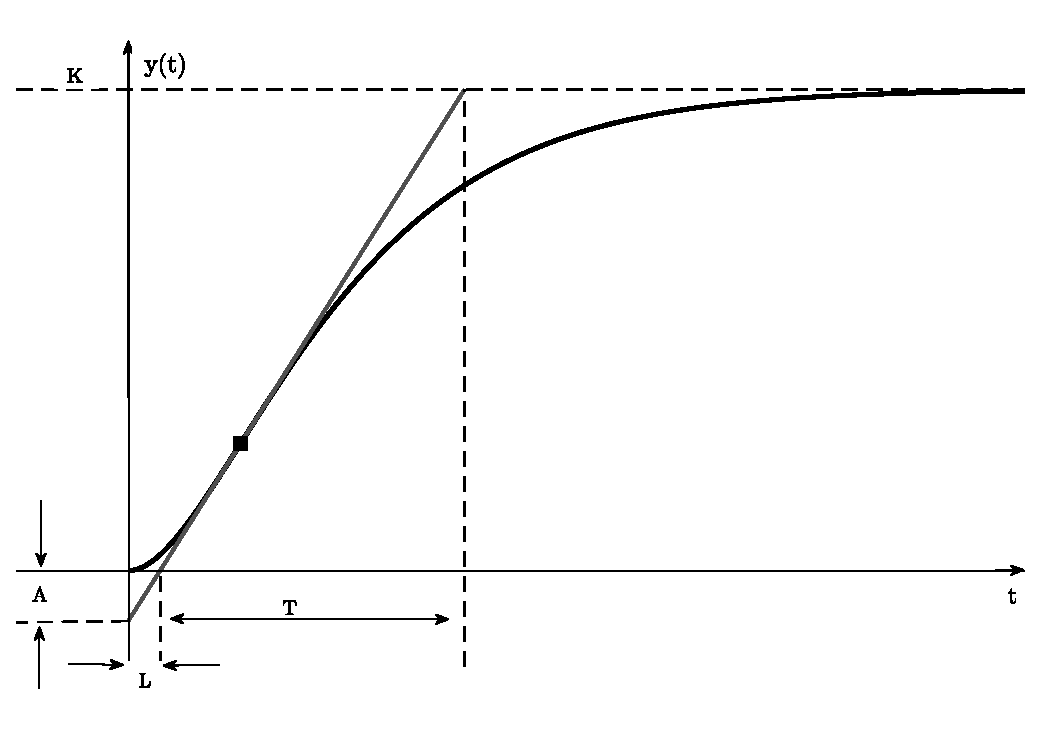
\includegraphics[width=0.5\textwidth]{figs/ZNol}
\caption{Respuesta escal�n en forma de \emph{s} del m�todo en lazo abierto}\label{ZNol}
\end{figure}
% ------------------------------------------------------------------------
Una vez obtenidos los valores importantes para cada caso, los par�metros del controlador PI (i.e. ganancia proporcional $k_P$ y tiempo integral $T_I$) se determinan con base en las equivalencias presentadas en la Tabla \ref{table_PI}.\\

% ------------------------------------------------------------------------
\begin{table}[htbp]
\caption[C�lculo controlador PI m�todos de \emph{Ziegler \& Nichols}]{Equivalencias c�lculo controlador PI para m�todos de \emph{Ziegler \& Nichols}}\label{table_PI}
	\centering
    \begin{threeparttable}
	\begin{tabular}{ c  c  c }
    \hline
    M�todo                       & $k_P$               & $T_I$                  \\ \hline
    \multicolumn{1}{c}{Lazo abierto}      & $0.45k_{cr}$        & $\frac{1}{1.2}P_{cr}$  \\
    \multicolumn{1}{c}{Lazo cerrado}      & $0.9 \frac{T}{L}$   & $\frac{L}{0.3}$        \\ \hline
	\end{tabular}
% ------------------------------------------------------------------------
\begin{tablenotes}
\scriptsize
\item[ ] \emph{Nota:} Adaptado de \citep{ogata2010}.
\end{tablenotes}
% ------------------------------------------------------------------------
\end{threeparttable}
\end{table}
% ------------------------------------------------------------------------

En el caso particular de una configuraci�n realimentada como la presentada en la Fig. \ref{sistem2ord} para la combinaci�n de planta y controlador dada respectivamente por las expresiones \eqref{plantaCPI} y \eqref{PIconteq}, es posible mostrar que el lugar geom�trico de las ra�ces para el sistema realimentado cruza el eje imaginario cuando $k_P = k_{cr} = 30$, con oscilaciones sostenidas de periodo $P_{cr} = 2.81 \: [s]$.\\

De esta manera, el controlador dise�ado corresponde con $k_P = 13.50$; $T_I = 2.34$; es decir:
% ------------------------------------------------------------------------
\begin{eqnarray}
\nonumber C(s) & = & 13.50 \left( 1 + \frac{1}{2.34 s}\right)\\
               & = & \frac{13.50s + 5.76}{s}
               \label{PIconteqval}.
\end{eqnarray}\
% ------------------------------------------------------------------------

Los par�metros de respuesta para el sistema compensado empleando dicho controlador, corresponden con:
$$
Mp = 104.05 \: [\%]; \quad t_s = 249.54 \: [s],
$$

seg�n ilustrado en la respuesta escal�n de la Fig. \ref{step_PI}.\\

Esta respuesta din�mica a pesar de ser estable, no representa un resultado
satisfactorio en t�rminos de velocidad de convergencia hacia el valor de estado estacionario, dadas las evidentes oscilaciones del r�gimen transitorio y el prolongado tiempo de establecimiento. Dicha condici�n es susceptible de mejora a trav�s de un \emph{ajuste fino}. N�tese sin embargo, que la acci�n de control es simple (PI) y la planta es de un orden significativo (tercero).\\

% ------------------------------------------------------------------------
\begin{figure}[h]
\centering
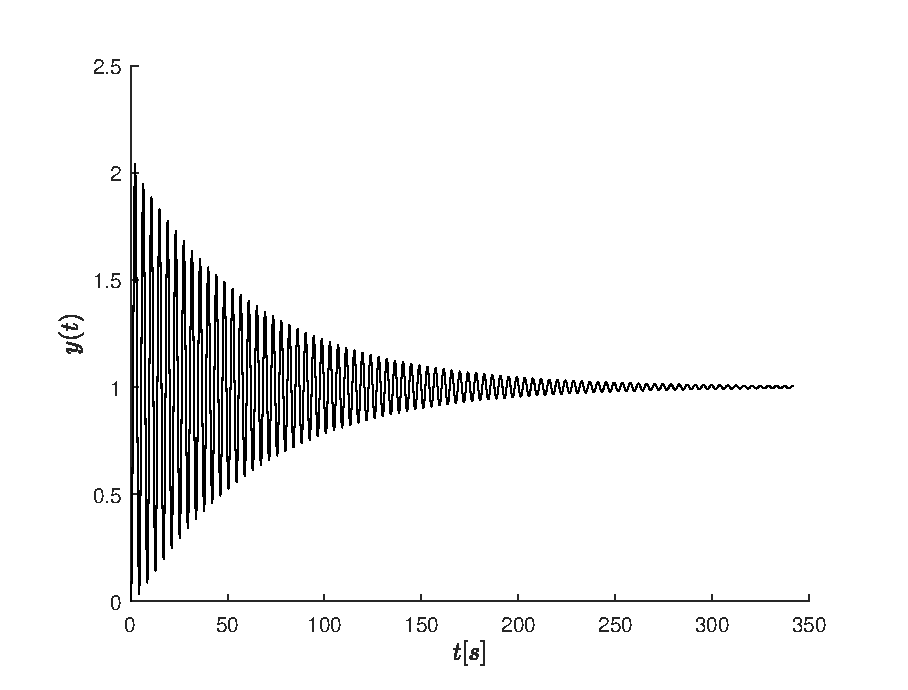
\includegraphics[width=0.5\textwidth]{figs/step_PI}
\caption{Respuesta escal�n del sistema compensado}\label{step_PI}	
\end{figure}

% ------------------------------------------------------------------------
\subsection{Conjunto estabilizante para sistema ante control PI}\label{conjestabpi}
% ------------------------------------------------------------------------
\noindent Empleando un tratamiento similar al utilizado para el an�lisis del conjunto estabilizante de la \emph{Secci�n} \ref{estabsect}, es posible deducir que la combinaci�n de planta + controlador definida en \eqref{plantaCPI} y \eqref{PIconteq}, permite delimitar una regi�n de estabilidad en el plano ($k_P$, $k_I$) dada por:
% ------------------------------------------------------------------------
\begin{eqnarray}
0 & < & k_{P} < 30; \label{stabsetPI1} \\
0 & < & k_{I} < \frac{-k_{P}^{2}+30k_{P}}{36},\label{stabsetPI2}
\end{eqnarray}
% ------------------------------------------------------------------------
definiendo a su vez el siguiente conjunto estabilizante:
\begin{equation}
\mathcal{S} = \left\{\left(k_P, k_I\right): \: \text{\eqref{stabsetPI1} y \eqref{stabsetPI2} se satisfagan simult�neamente} \right\}.\label{stabsetPIeq}
\end{equation}
% ------------------------------------------------------------------------
La Fig. \ref{Stab_set_PI} ilustra el conjunto estabilizante \eqref{stabsetPIeq}, resaltando en su interior mediante un asterisco el punto correspondiente al controlador dise�ado y definido en \eqref{PIconteqval}.\\
% ------------------------------------------------------------------------
\begin{figure}[h]
\centering
\includegraphics[width=0.5\textwidth]{figs/stab_set_PI}
\caption{Conjunto estabilizante en el plano ($k_P$, $k_I$)}\label{Stab_set_PI}
\end{figure}
% ------------------------------------------------------------------------

Como se observa, el controlador analizado en la Fig.\ref{step_PI} se encuentra cerca de los l�mites de estabilidad, justificando la alta oscilaci�n de su respuesta din�mica.\\

La siguiente \emph{Secci�n} realizar� un an�lisis alrededor de la \emph{fragilidad} del controlador PI.

% ------------------------------------------------------------------------
\section{Fragilidad de controladores PI}
% ------------------------------------------------------------------------
\noindent Los m�todos de \emph{Ziegler \& Nichols} para la sintonizaci�n de controladores PI y PID
han sido la referencia empleada por ingenieros en diversos campos de aplicaci�n desde su
aparici�n en 1942. Sin embargo, como se observ� en el ejemplo presentado en la \emph{Secci�n} anterior, no siempre se logra una respuesta din�mica adecuada a las exigencias
de una respuesta deseada, aunque la misma sea estable.\\

La forma tradicional de corregir esta situaci�n, es considerar que los par�metros del
controlador PI o PID obtenidos por el m�todo de \emph{Ziegler \& Nichols} son el valor inicial
de un proceso iterativo denominado \emph{ajuste fino}, que permitir� eventualmente obtener
una respuesta mejorada en t�rminos de \emph{nuevos valores sintonizados}.\\

El objetivo de la presente \emph{Secci�n} no es discutir el proceso de sinton�a fina de par�metros en los m�todos de Ziegler \& Nichols, sino evaluar la \emph{fragilidad del controlador} dise�ado con dicho m�todo, en t�rminos
de su conjunto estabilizante.\\

En \citep{Bhatt97} Bhattacharyya define la \emph{fragilidad de un controlador} como aquel fen�meno que implica para el mismo m�rgenes de estabilidad extremadamente peque�os. Otra manera de entender el concepto es a trav�s de la m�s peque�a perturbaci�n admisible en los par�metros de un controlador tal que el sistema realimentado pierda su estabilidad. La fragilidad es un concepto muy cercano a la robustez, y  por tanto conviene enfatizar en que la primera estudia la manera en que alteraciones leves en los valores de par�metro de un controlador afectan la estabilidad del sistema realimentado, mientras que la segunda realiza el estudio independientemente de donde hayan ocurrido las variaciones param�tricas.

% ------------------------------------------------------------------------
\subsection{Geometr�a para m�rgenes de estabilidad en un controlador PI}\label{margeom}
% ------------------------------------------------------------------------
\noindent Una interpretaci�n geom�trica del margen de fase para un sistema
realimentado ante un control PI, se propone en \citep{Alzate2016}. El desarrollo presentado en el presente numeral se basa en el trabajo referenciado
y sugiere la manera de aplicar el mismo resultado en t�rminos del margen de ganancia del sistema.\\

Para ello, asuma $P(j\omega)$ y $C(j\omega)$ como la respuesta frecuencial de la planta y el controlador PI definidos en \eqref{plantaCPI} y \eqref{PIconteq}, respectivamente. En el sistema realimentado estable que se obtiene a partir de esta combinaci�n \emph{planta + controlador}, los m�rgenes de ganancia $A_m$ y fase $\theta_m$ se pueden determinar anal�ticamente a partir de las condiciones de magnitud y fase:
% ------------------------------------------------------------------------
\begin{equation}
 |P(j\omega_g)||C(j\omega_g)| =1, \label{CondMag}
\end{equation}
% ------------------------------------------------------------------------
% ------------------------------------------------------------------------
\begin{equation}
\angle{P(j\omega_{\theta})}+\angle{C(j\omega_{\theta})}={\pi}n; \quad n=\pm 1,3,5... \label{Condpha}
\end{equation}
% ------------------------------------------------------------------------
de manera que:
% ------------------------------------------------------------------------
\begin{equation}
A_m=\frac{1}{|P(j\omega_{\theta})||C(j\omega_{\theta})|}, \label{Am}
\end{equation}
% ------------------------------------------------------------------------
% ------------------------------------------------------------------------
\begin{equation}
\theta_m=\angle{P(j\omega_{g})}+\angle{C(j\omega_{g})}-\pi, \label{pm}
\end{equation}
% ------------------------------------------------------------------------
siendo $w_g$ y $w_{\theta}$ las frecuencias de cruce de ganancia y fase, respectivamente.\\

Alternativamente, estos margenes de estabilidad pueden obtenerse a partir de una relaci�n geom�trica en el plano de par�metros $\left(k_P, k_I\right)$ de un controlador PI, con respecto al conjunto estabilizante $\mathcal{S}$ de la planta bajo esta acci�n de control.\\

As� entonces, tomando en cuenta que:
% -----------------------------------------------------------------------
\begin{eqnarray}
\nonumber C(j \omega) & = & k_P + \frac{k_I}{j \omega}\\
                      & = & k_P - \frac{k_I}{\omega}j,
\end{eqnarray}
% -----------------------------------------------------------------------
la fase del controlador PI puede expresarse como:
% ------------------------------------------------------------------------
\begin{eqnarray}
\angle{C(j\omega)} & = & \arctan{\left(\frac{-k_I}{{\omega}k_P}\right)} \label{phi_c},
\end{eqnarray}
% ------------------------------------------------------------------------
o equivalentemente:
% ------------------------------------------------------------------------
\begin{eqnarray}
-\omega{k_P}\tan\left(\angle{C(j\omega)}\right) & = & k_I. \label{recta}
\end{eqnarray}\
% ------------------------------------------------------------------------

Si en la expresi�n anterior se asume $\omega = \omega_g$, la fase del controlador $\angle{C(j\omega_{g})}$ debe satisfacer un margen de fase $\theta_m$ ante una respuesta frecuencial $P(j \omega)$ conocida para la planta, seg�n definido en \eqref{pm}. Por tanto, ante esta situaci�n la expresi�n \eqref{recta} define una linea recta en el plano $\left(k_P, k_I\right)$ con pendiente $-\omega{\tan\left(\angle{C(j\omega)}\right)}$, cuyos puntos satisfacen dichas restricciones.\\

Asimismo, a partir de la condici�n de magnitud del controlador se tiene:
% ------------------------------------------------------------------------
\begin{eqnarray}
{|C(j\omega)|}^2 & = & {k_P}^{2}+\frac{{k_I}^{2}}{\omega^{2}}, \label{M_c^2}
\end{eqnarray}
% ------------------------------------------------------------------------
o equivalentemente:
% ------------------------------------------------------------------------
\begin{eqnarray}
\frac{{k_P}^{2}}{{|C(j\omega)|}^2}+\frac{{k_I}^{2}}{{|C(j\omega)|}^2{\omega}^2} & = & 1. \label{elipse}
\end{eqnarray}\
% ------------------------------------------------------------------------

Bajo la misma suposici�n de $\omega = \omega_g$, la expresi�n anterior representar� una elipse en el plano $\left(k_P, k_I\right)$, que intersecta a la recta \eqref{recta} seg�n ilustrado en el diagrama de la Fig.~\ref{curvas1}.\\

El punto de intersecci�n, dar� la coordenada $\left(k_P, k_I\right)$ del controlador PI que satisface $\theta_m$ y $\omega_g$, representando un m�todo gr�fico para el dise�o de controladores.\\

Al respecto del m�todo se resaltan los siguientes detalles adicionales:
\begin{itemize}
\item[-] La intersecci�n entre la elipse y la linea recta se da para dos puntos del plano. Sin embargo, puede observarse de la Fig.~\ref{curvas1} que s�lo uno de ellos tiene sentido pr�ctico por encontrarse al interior del conjunto estabilizante $\mathcal{S}$;
\item[-] La magnitud para $C\left(j \omega_g\right)$ se deja como un par�metro libre de dise�o y de este depende la amplitud (i.e. radio mayor y radio menor) de la elipse en el plano;
\item[-] El margen de ganancia no se involucra expl�ticamente en el m�todo sugerido, aunque se entiende que la elecci�n arbitraria para $|C\left(j \omega_g\right)|$ influencia dicho valor. La Secci�n siguiente abordar� con mayor detalle este aspecto;
\item[-] El procedimiento sugerido puede abordarse expl�citamente desde el margen de ganancia, seleccionando $\omega = \omega_\theta$ y forzando de \eqref{Am} a la magnitud del controlador $|C(j\omega_{\theta})|$ a satisfacer un margen de ganancia $A_m$ ante una respuesta frecuencial $P(j \omega)$ conocida para la planta. Ante esta situaci�n, el punto de intersecci�n en el plano $\left( k_P, k_I \right)$ para la elipse y la linea recta representar� la coordenada $\left(k_P, k_I\right)$ del controlador PI que satisface $A_m$ y $\omega_\theta$, dejando como par�metro libre a la pendiente de la recta y a trav�s de ella, al margen de fase para el sistema controlado.
\end{itemize}
% ------------------------------------------------------------------------
\begin{figure}
\centering
	\subfigure[]{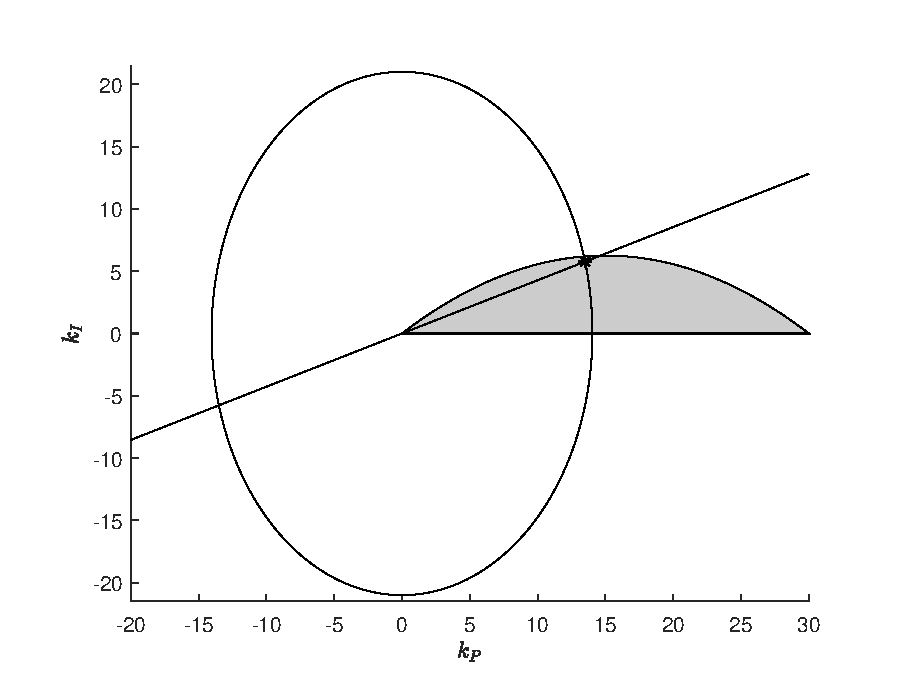
\includegraphics[width=0.5\textwidth]{Figs/curvas1}}
	\subfigure[]{\includegraphics[width=0.5\textwidth]{Figs/curvas1-2}}
\caption[Intersecci�n en el plano $\left( k_P, k_I \right)$ para linea recta y elipse]{Intersecci�n en el plano $\left( k_P, k_I \right)$ para linea recta y elipse, dados $\omega = \omega_g$ y $\theta_m$, ilustrando: (a) panor�mica general de la intersecci�n y (b) detalle del punto de intersecci�n}\label{curvas1}
\end{figure}
% ------------------------------------------------------------------------

\subsection{Definici�n de m�trica para calcular distancia a inestabilidad}\label{metrdef}
% ------------------------------------------------------------------------
\noindent Como ya definido al principio de la presente \emph{Secci�n}, un buen dise�o para un controlador debe ir
m�s all� de la simple respuesta din�mica del sistema controlado y por tanto, debe adem�s garantizar
la estabilidad para el lazo de control a�n ante leves variaciones en sus
par�metros.\\

Complementando las ideas de \emph{Bhattacharyya y Keel} en \citep{Bhatt97}, se emplear� la visi�n geom�trica
propuesta por \emph{Morarescu et al} adaptada en el presente documento para
el caso de lazos PI sin retardo \citep{Mendez2008} \citep{Morarescu2010}.\\

Para ello, se define la distancia eucl�dea:
% ------------------------------------------------------------------------
\begin{equation}
d = \sqrt{(k_P^*-k_P)^2+(k_I^*-k_{I})^2},\label{d}
\end{equation}
% ------------------------------------------------------------------------
siendo $\left(k_P^*, k_I^* \right)$ las coordenadas para un controlador en el l�mite del conjunto estabilizante $\mathcal{S}$ y ortogonal a $\left(k_P, k_I \right)$, que define el radio para una circunferencia de puntos que representan un rango o margen de estabilidad.\\

A partir de lo anterior, dado un controlador PI al interior de $\mathcal{S}$ es posible cuantificar su \emph{fragilidad} a trav�s de esta m�trica, al menos en un modo relativo; es decir, dados dos controladores estables ser� m�s \emph{fr�gil} aquel para el cual se obtenga el menor $d$.\\

Sin embargo, no es claro el significado de \emph{fragilidad} para un valor $d$ en un contexto absoluto.\\

En cualquier caso, el c�lculo para $d$ en \eqref{d} implica conocer las coordenadas del punto $\left(k_P^*, k_I^* \right)$. Dichas coordenadas representan un valor en la frontera de $\mathcal{S}$, que conecta con el punto de an�lisis $\left(k_P, k_I \right)$ a trav�s de una l�nea recta y por tanto, en teor�a habr� una soluci�n para $\left(k_P^*, k_I^* \right)$ en cada direcci�n posible de proyecci�n para el vector $\left(k_P^*-k_P, k_I^*-k_I \right)$ en el plano. En \citep{Mendez2008} \citep{Morarescu2010} por ejemplo, los resultados presentados se realizan a partir de una proyecci�n sobre la vertical. Una soluci�n m�s general implica el m�nimo valor para $d$ en un barrido de $360�$ lo cual no es trivial, al menos anal�ticamente, si se piensa en que la descripci�n para la frontera de $\mathcal{S}$ corresponde con funciones definidas por tramos (es decir, con transiciones condicionadas).\\

Como alternativa, se presenta en el presente apartado una forma de calcular dicho punto l�mite a partir del enfoque geom�trico discutido en la \emph{Secci�n} \ref{margeom}. Para ello, considere el problema de cuantificar la fragilidad del controlador PI calculado en \eqref{PIconteqval}.\\

Dicho controlador representa un punto en el conjunto estabilizante $\mathcal{S}$ en \eqref{stabsetPIeq} y a su vez, la intersecci�n entre una l�nea recta y una elipse dadas respectivamente por \eqref{recta} y \eqref{elipse}, con los siguientes par�metros: $\omega_g = 1.49 \: rad/s$ y $\theta_m = 1.18�$ (el c�lculo para dichos par�metros fue realizado empleando la funci�n \emph{allmargins(.)} de MATLAB).\\

En t�rminos pr�cticos, la regla de dise�o indica que un buen margen de fase es alrededor de $60�$ \citep{Hang1992}. Como se observa el margen de fase $\theta_m$ obtenido por \emph{Ziegler \& Nichols} es muy cercano a la inestabilidad y por tanto sugiere \emph{fragilidad}.\\

Para determinar los valores l�mite $\left(k_P^*, k_I^* \right)$, se mantiene constante la pendiente de la recta \eqref{recta} a la misma frecuencia $\omega=\omega_g = 1.49 \: rad/s$ y se incrementa la amplitud de la elipse \eqref{elipse} a partir del par�metro $|C\left(j \omega_g\right)|$ (ver Fig.\ref{curvas2a}).\\

Ante estas condiciones, el margen de ganancia $A_m$ del sistema puede determinarse mediante el cociente entre las distancias eucl�deas correspondientes a los puntos $\left(k_P, k_I \right)$ y $\left(k_P^*, k_I^* \right)$; es decir \citep{Diaz2016}:
% ------------------------------------------------------------------------
\begin{eqnarray}
\nonumber A_m & = & \frac{\sqrt{\left(k_P^*\right)^2 + \left(k_I^*\right)^2}}{\sqrt{\left(k_P\right)^2 + \left(k_I\right)^2}}\\
\nonumber     & = & \frac{\sqrt{\left(k_P^*\right)^2 + \left(-\omega{k_P^*}\tan\left(\angle{C(j\omega)}\right)\right)^2}}{\sqrt{\left(k_P\right)^2 + \left(-\omega{k_P}\tan\left(\angle{C(j\omega)}\right)\right)^2}}\\
\nonumber     & = & \frac{k_P^*\sqrt{1 + \left(-\omega\tan\left(\angle{C(j\omega)}\right)\right)^2}}{k_P\sqrt{1 + \left(-\omega\tan\left(\angle{C(j\omega)}\right)\right)^2}}\\
\nonumber     & = & \frac{k_P^*}{k_P}\\
    & = & \frac{k_I^*}{k_I}.\label{margeng}
\end{eqnarray}\
% ------------------------------------------------------------------------

De este resultado se observa que si $\left(k_P, k_I \right)$ se encuentra en la frontera de $\mathcal{S}$ entonces $A_m = 1$; si $\left(k_P, k_I \right)$ se encuentra fuera  de $\mathcal{S}$ entonces $A_m < 1$ y si $\left(k_P, k_I \right)$ se encuentra dentro de $\mathcal{S}$ entonces $A_m > 1$, lo cual coincide con el comportamiento esperado
seg�n la teor�a para dicho margen en t�rminos de la estabilidad del sistema.\\

De esta manera, igualando \eqref{recta} para $k_I$ con la condici�n de frontera dada por \eqref{stabsetPI2}, se obtiene:
% ------------------------------------------------------------------------
\begin{eqnarray}
\nonumber -\omega_g {k_P^*}\tan\left(\angle{C(j\omega_g)}\right) & = & \frac{-\left(k_P^*\right)^{2}+30k_P^*}{36}\\
\nonumber \left(k_P^*\right)^{2}-30k_P^*-36\omega_g {k_P^*}\tan\left(\angle{C(j\omega_g)}\right) & = & 0\\
\nonumber \left(k_P^*\right)^{2}-30k_P^*-53.64{k_P^*}\tan\left(-0.2789\right) & = & 0\\
\nonumber \left(k_P^*\right)^{2}-30k_P^*+15.36{k_P^*} & = & 0\\
k_P^*\left(k_P^* - 14.64\right) & = & 0,
\end{eqnarray}\
% ------------------------------------------------------------------------
tras reemplazar los valores conocidos para $\omega_g$, $k_P$ y $k_I$. A partir de ello, $k_P^* = 14.64$ corresponde con la soluci�n v�lida en el conjunto estabilizante $\mathcal{S}$ mostrado previamente en la Fig.\ref{Stab_set_PI}. Dicho valor evaluado en:
% ------------------------------------------------------------------------
\begin{eqnarray}
\nonumber k_I^* & = & -\omega_g {k_P^*}\tan\left(\angle{C(j\omega_g)}\right)\\
                & = & 6.24,
\end{eqnarray}\
% ------------------------------------------------------------------------
permite obtener como coordenada de frontera: $\left(k_P^*, k_I^* \right) = \left(14.64, 6.24 \right)$ y por ende, un margen de ganancia:
\begin{eqnarray*}
% ------------------------------------------------------------------------
A_m & = & \frac{14.64}{13.50}\\
    & = & \frac{6.24}{5.76}  \\
    & = & 1.08,
\end{eqnarray*}\
% ------------------------------------------------------------------------
para el controlador \eqref{PIconteqval}, que a su vez representa una distancia (ver Fig.\ref{distancia}):
% ------------------------------------------------------------------------
\begin{eqnarray*}
d & = & \sqrt{(14.64-13.50)^2+(6.24-5.76)^2}\\
& = & 1.2369.
\end{eqnarray*}
% ------------------------------------------------------------------------
Como se observa, el valor de $d$ por s� solo no es tan diciente como los m�rgenes de estabilidad $A_m$ y $\theta_m$ obtenidos, ambos de valor muy peque�o.\\

Una formulaci�n similar podr�a haberse realizado calculando a partir de \eqref{PIconteqval} el valor de $A_m$ y $\omega_\theta$, y con base en ello determinar los valores l�mite $\left(k_P^*, k_I^* \right)$ tras mantener constante la amplitud de la elipse modificando la pendiente de la recta hasta alcanzar la frontera del conjunto estabilizante $\mathcal{S}$, y a trav�s de ello el margen de fase $\theta_m$ para el sistema (ver Fig.\ref{curvas2b}).\\

Finalmente, se debe mencionar que la interfaz desarrollada en la \emph{Secci�n} \ref{interfazsect} fue complementada incorporando el c�lculo gr�fico para controladores PI, junto con una determinaci�n para sus m�rgenes de estabilidad y para la distancia $d$, como medida de su \emph{fragilidad}.
% ------------------------------------------------------------------------
\begin{figure}
\centering
	\subfigure[]{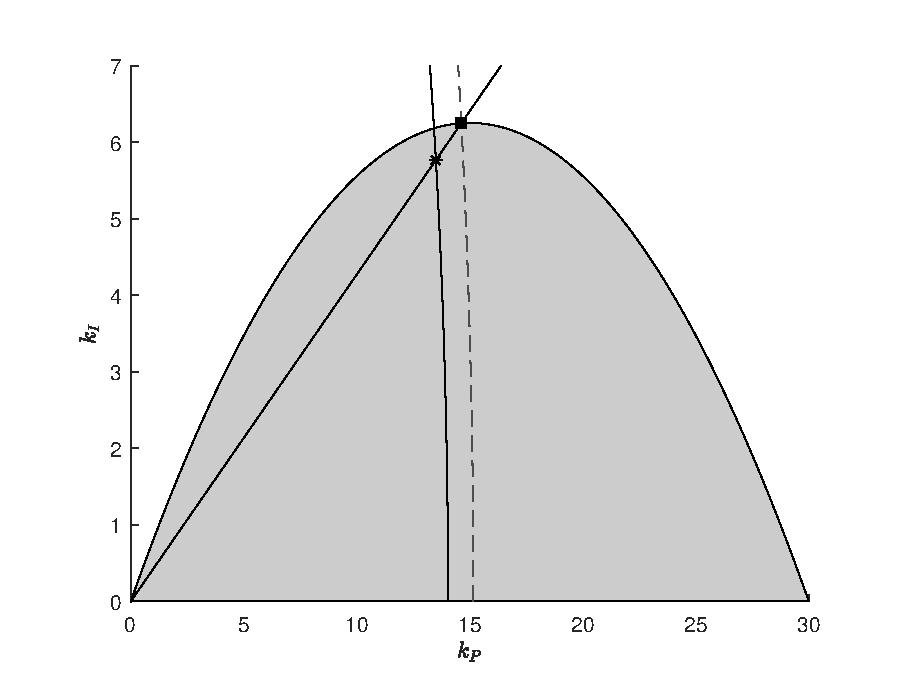
\includegraphics[width=0.5\textwidth]{Figs/curvas2-1}\label{curvas2a}}
	\subfigure[]{\includegraphics[width=0.5\textwidth]{Figs/curvas2-2}\label{curvas2b}}
\caption[Representaci�n en $\left(k_P, k_I \right)$ para m�rgenes de estabilidad]{Representaci�n geom�trica en el plano $\left(k_P, k_I \right)$ para m�rgenes de estabilidad: (a) $A_m$ manteniendo fija la recta y variando la elipse; (b) $\theta_m$ manteniendo fija la elipse y variando la recta}\label{curvas2}
\end{figure}
% ------------------------------------------------------------------------
\begin{figure}
\centering
	\subfigure[]{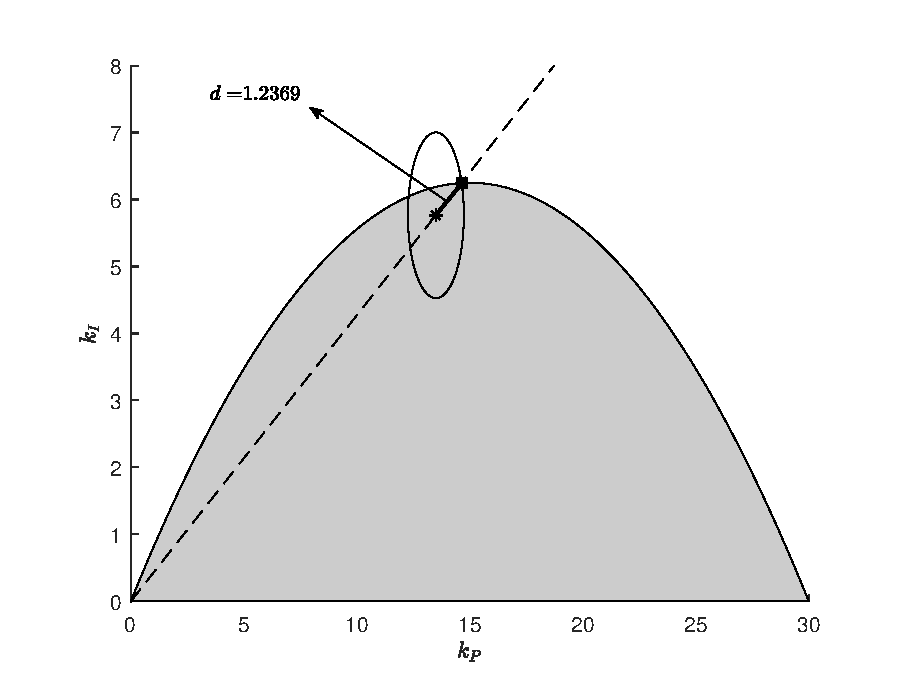
\includegraphics[width=0.5\textwidth]{Figs/max_dist_2}}
	\subfigure[]{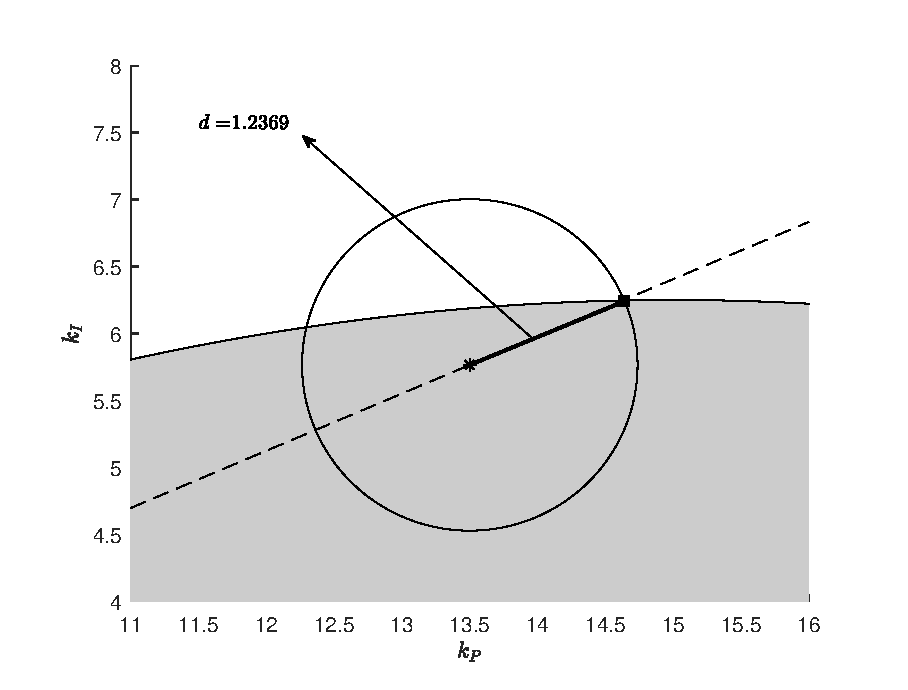
\includegraphics[width=0.5\textwidth]{Figs/max_dist}}
\caption[Distancia a la inestabilidad]{Distancia a la inestabilidad ilustrando: (a) panor�mica general de la m�trica y (b) detalle de la m�trica}\label{distancia}
\end{figure}
% ------------------------------------------------------------------------   	% Marco t�cnico
% ------------------------------------------------------------------------
% ------------------------------------------------------------------------
% ------------------------------------------------------------------------
%                            Recomendaciones
% ------------------------------------------------------------------------
% ------------------------------------------------------------------------
% ------------------------------------------------------------------------

\chapter{Desarrollo del proyecto}
% ------------------------------------------------------------------------
\noindent En este Cap�tulo se presentar� como fue desarrollado el proyecto.
% ------------------------------------------------------------------------ 
\section{Ambientaci�n tecnol�gica}
\subsection{Investigaci\'on fundamentos te\'oricos relacionados con el proyecto (Tecnolog\'ias y est\'andares)}
Durante esta primera fase se investig� el estado del arte en cloud computing para poder identificar los conceptos comunes en las diferentes arquitecturas cloud enfocadas a IoT. De esta primera fase se encontr� la gesti�n de contenedores como factor com�n por lo cual la investigaci�n posterior sigui� este enfoque. Posteriormente se identificaron las tecnolog�as mas populares en IoT.

\begin{table}[H]
	\begin{minipage}{1\textwidth}
		\caption[Tecnolog�as disponibles en el mercado]{ \raggedright Tecnolog�as disponibles en el mercado}
		\label{tabla:Tecnolog�as disponibles en el mercado}
		\begin{center}
			\begin{tabular}{ p{5cm}   p{5cm}  p{5cm}  }
				\hline
				Sistema Operativo & Container Runtime & Orquestador de contenedores \\
				\hline
				CentOS & Cri-O & Apache Mesos \\
				CoreOS & Docker & Docker Swarm \\
				Red Hat Enterprise Linux & Linux VServer & Kontena \\
				Oracle Linux & LXD & Kubernetes \\
				Ubuntu Server & Rkt  & Nomad \\
				Windows Server & Windows Containers & Openstack Magnum x
				\\ \hline
			\end{tabular}
		\end{center}
	\end{minipage}
\end{table}

A medida que se desarroll� en proyecto, nuevas tecnolog�as fueron a�adidas al stack pero ya de eso se hablar� mas adelante en el documento.

A medida que se desarroll� en proyecto, nuevas tecnolog�as fueron a�adidas al stack pero ya de eso se hablar� mas adelante en el documento.

\subsection{Estudio}
Durante esta etapa se realiz� una revisi�n general sobre cada una de las tecnolog�as, lo cual sirvi� de base para la definir los criterios de selecci�n para realizar un primer filtro sobre las tecnolog�as a usar en la infraestructura en la siguiente etapa.

\begin{itemize}
	\item Licencia
	\item Stacks
	\item Soporte
	\item Uso libre en producci�n
\end{itemize}



\subsection{Sondeo}
Durante esta etapa se aplicaron los diferentes criterios entre cada una de las tecnolog�as y se consolido est� informaci�n en las tablas \ref{tabla:Sondeo de selecci�n: Sistema Operativo}, \ref{tabla:Sondeo de selecci�n: Container Runtime} y \ref{tabla:Sondeo de selecci�n: Orquestador de contenedores}.
\begin{table}[H]
	\begin{minipage}{1\textwidth}
		\caption[Sondeo de selecci�n: Sistema Operativo]{ \raggedright Sondeo de selecci�n: Sistema Operativo}
		\label{tabla:Sondeo de selecci�n: Sistema Operativo}
		\begin{center}
			\begin{tabular}{ p{3cm}   p{3cm}  p{2cm}  p{3cm}  p{4cm}  }
				\hline
				S. Operativo & Licencia & Stacks & Soporte & Gratis en producci�n \\  \hline
				CentOS & GPL & 1.85K & Comunidad & Si
				\\ 
				CoreOS & Apache 2.0 & 164 & Comunidad & Si
				\\ 
				RHEL\footnote{Red Hat Enterprise Linux} & GPL\footnote{Solo para efectos de desarrollo, en producci�n se cobra una tarifa.} & - & Privado & No
				\\ 
				Oracle Linux & GPL & - & Privado & Si
				\\ 
				Ubuntu Server & GPL & 9.1k & Hibrido\footnote{Posibilidad de adquirir soporte pago pero posee una gran comunidad que lo respalda.} & Si
				\\ 
				Windows Server & M�ltiple\footnote{Microsoft provee diferentes licencias seg�n los servicios solicitados.} & 3.4k & Privado & No
				\\ \hline
			\end{tabular}
		\end{center}
		{La cantidad de stacks fueron tomados de: \url{https://stackshare.io/}}
	\end{minipage}
\end{table}


\begin{table}[H]
	\begin{minipage}{1\textwidth}
		\caption[Sondeo de selecci�n: Container Runtime]{ \raggedright Sondeo de selecci�n: Container Runtime}
		\label{tabla:Sondeo de selecci�n: Container Runtime}
		\begin{center}
			\begin{tabular}{ p{3cm}  p{3cm} p{2cm}  p{4cm}  p{3cm}  }
				\hline
				Container Runtime & Licencia & Stacks & Soporte & Uso libre en producci�n \\ \hline
				Cri-O & Apache 2.0 & - & Comunidad & Si
				\\ 
				Docker & Apache 2.0 & 16.6K & Comunidad/Privado & Si
				\\ 
				Linux VServer & GPL & - & Comunidad & Si
				\\ 
				LXD & Apache 2.0 & 39 & Comunidad & Si
				\\ 
				Rkt & Apache 2.0 & 21 & Comunidad & Si
				\\
				Windows Containers & SaaS & - & Privado & No
				\\ \hline
			\end{tabular}
		\end{center}
		{La cantidad de stacks fueron tomados de:
			\url{https://stackshare.io/}}
	\end{minipage}
\end{table}


\begin{table}[H]
	\begin{minipage}{1\textwidth}
		\caption[Sondeo de selecci�n: Orquestador de contenedores]{ \raggedright Sondeo de selecci�n: Orquestador de contenedores}
		\label{tabla:Sondeo de selecci�n: Orquestador de contenedores}
		\begin{center}
			\begin{tabular}{ p{3cm}   p{3cm}  p{2cm}  p{4cm}  p{3cm}  }
				\hline
				Orquestador & Licencia & Stacks & Soporte & Gratis en producci�n \\ \hline
				Apache Mesos &  Apache 2.0 & 177 & Comunidad & Si 
				\\ \hline
				Docker Swarm & Apache 2.0  
				\footnote{Algunos componentes se encuentran bajo la licencia Apache 2.0 y otros bajo Docker Enterprise 2.0 y 2.1} & 319 & Comunidad/Privado & Si\footnote{Si se desea utilizar Docker Trusted Registry o Universal Control Pane, si es necesario adquirir una licencia.}
				\\ 
				Kontena & Apache 2.0 & 7 & Comunidad & Si
				\\ 
				Kubernetes & Apache 2.0 & 4.25k & Comunidad & Si 
				\\ 
				Nomad & Mozilla 2.0 & 56 & Comunidad/Privado & Si \footnote{HashiCorp ofrece planes pagos con funcionalidades adicionales}
				\\ 
				Docker Compose & Apache 2.0 & 3.19k\footnote{Se utiliz� la cantidad de stacks de Openstack} & Comunidad/Privado & Si 
				\\ \hline
			\end{tabular}
		\end{center}
		{La cantidad de stacks fueron tomados de:
			\url{https://stackshare.io/}}
	\end{minipage}
\end{table}






   	% Desarrollo del proyecto
% ------------------------------------------------------------------------
% ------------------------------------------------------------------------
% ------------------------------------------------------------------------
%                            Trabajo futuro
% ------------------------------------------------------------------------
% ------------------------------------------------------------------------
% ------------------------------------------------------------------------

\chapter{Trabajo futuro}
% ------------------------------------------------------------------------
\noindent Actividades complementarias a los desarrollos presentados, incluyen el c�lculo autom�tico para conjuntos estabilizantes en plantas arbitrarias empleando el \emph{m�todo de la signatura} desarrollado por Keel y Bhattacharyya en \citep{keel2008}.\\

Asimismo es importante explorar otras topologias de compensador y controladores PID, en sus versiones de tiempo continuo y discreto.
% ------------------------------------------------------------------------    	% Conclusiones
% ------------------------------------------------------------------------
% ------------------------------------------------------------------------
% ------------------------------------------------------------------------
%                             Conclusiones
% ------------------------------------------------------------------------
% ------------------------------------------------------------------------
% ------------------------------------------------------------------------

\chapter{Recomendaciones}

\begin{itemize}
	\item Explorar los diferentes plugins que ofrece la comunidad de Openshift Origin.
	\item Utilizar servidores con las caracter�sticas recomendadas por la documentaci�n de Openshift Origin.
	\item Hacer uso de discos duros de estado s�lido con el fin de aumentar el rendimiento en los puntos en que es necesario acceder al disco, por ejemplo, las consultas hechas a la base de datos.
	\item Hacer uso de bases de datos distribuidas para poder realizar un escalamiento proporcional a la cantidad de pods. Tener en cuenta que el conector usado en el backend puede cambiar.
	\item Hacer la instalaci�n de los diferentes componentes directamente sobre las m�quinas y no recurrir a la virtualizaci�n como fue necesario durante la implementaci�n del prototipo.
	\item Conectar los servidores por 10 Gigabit Ethernet en lugar de Gigabit Ethernet.
	\item Con el fin de minimizar los riesgos durante un fallo el�ctrico, ser�a de ayuda a�adir una UPS a la infraestructura.
	\item Hacer uso de un sistema de almacenamiento en la nube (AWS, GCP, Azure o DigitalOcean).
	\item Instalar un registro de Docker privado para guardar las im�genes.
	\item Implementar End to End testing.
\end{itemize}   	% Recomendaciones
\input{Secs/T8}   	% Limitaciones
% ------------------------------------------------------------------------
% Bibliograf�a
% ------------------------------------------------------------------------
\addcontentsline{toc}{chapter}{Referencias Bibliogr�ficas}\newpage
\bibliographystyle{apalike}
\bibliography{xbib}
% ------------------------------------------------------------------------
% Anexos
% ------------------------------------------------------------------------

\newpage
\nnchapter{Ap�ndices}
% ------------------------------------------------------------------------
\anexo{Dataset generado para pruebas}\label{appendix:Dataset generado para pruebas}
El dataset fue generado en usando \href{https://mockaroo.com/}{mockaroo} con la siguiente configuraci�n:
\\
\includegraphics[width=\textwidth]{figs/moockaroo.png}
\\
Posteriormente, se exportaron 15 datasets en formato CSV que fueron concatenados debido a que mockaroo limita a 1000 la cantidad de filas en la versi�n gratuita. 

El archivo se encuentra en el siguiente link: \href{https://raw.githubusercontent.com/JoseDRojasA/thesis-files/master/Plan de pruebas/MOCK_DATA.csv}{Plan de pruebas/MOCK\_DATA.csv} % Fundamentos de s�lidos r�gidos

\newpage
\anexo{Archivo Inventory}\label{appendix:Archivo Inventory}
\begin{minted}[
	gobble=4,
	frame=single,
	linenos,
	breaklines
	]{yaml}
				[OSEv3:children]
				masters
				nodes
				etcd
				[OSEv3:vars]
				ansible_ssh_user=root
				openshift_deployment_type=origin
				openshift_master_identity_providers=[{'name': 'htpasswd_auth', 'login': 'true', 'challenge': 'true', 'kind': 'HTPasswdPasswordIdentityProvider'}]
				openshift_disable_check=memory_availability,disk_availability
				[masters]
				master1.local.cluster
				[etcd]
				master1.local.cluster
				[nodes]
				master1.local.cluster openshift_node_group_name='node-config-master-infra'
				node1.local.cluster openshift_node_group_name='node-config-compute'
				node2.local.cluster openshift_node_group_name='node-config-compute'
\end{minted} % Funci�n ode45 de MATLAB
% ------------------------------------------------------------------------
% ------------------------------------------------------------------------
% ------------------------------------------------------------------------
%                                Anexo C
% ------------------------------------------------------------------------
% ------------------------------------------------------------------------
% ------------------------------------------------------------------------
% ------------------------------------------------------------------------
\newpage
\anexo{Endpoints glusterfs}\label{appendix:Archivos de despliegue: Endpoints glusterfs}


    \begin{minted}[
gobble=4,
frame=single,
linenos,
breaklines
]{yaml}
				apiVersion: v1
				kind: Endpoints
				metadata:
				name: glusterfs-cluster
				subsets:
				- addresses:
				- ip: 192.168.0.133
				ports:
				- port: 1
				- addresses:
				- ip: 192.168.0.134
				ports:
				- port: 1
\end{minted}  
 % Interfaz de animaci�n de la din�mica del sistema
% ------------------------------------------------------------------------
\end{document}                                          % Fin de documento
% ------------------------------------------------------------------------ 